\documentclass[acmsmall,timestamp,review,anonymous]{acmart}

% Packages {{{
\usepackage{hyperref}
\usepackage{amsmath}
\usepackage{amssymb}
\usepackage{bbm}
\usepackage{tikz}
\usetikzlibrary{calc}
\usetikzlibrary{graphs}
\usetikzlibrary{cd}
\usepackage{bussproofs}
\usepackage{stmaryrd}
\usepackage{calc}
\usepackage{bbm}
% }}}

% Parameters {{{

\hyphenation{Comp-Cert}

% }}}

% Macros {{{

%\newtheorem{example}{Example}
%\newtheorem{definition}{Definition}
%\newtheorem{lemma}{Lemma}

\newcommand{\kw}[1]{\ensuremath{ \mathsf{#1} }}
\newcommand{\ifr}[1]{\ [{#1}]\ }
\newcommand{\ifrw}[2]{\ [{#1}]_{#2}\ }
\newcommand{\alt}{\ |\ } % use \mid instead
\newcommand{\bind}{\gg\!\!=}

\newcommand{\EC}{\kw{C}}
\newcommand{\simrel}{\kw{simrel}}

% Moves
\newcommand{\mcall}[3]{\kw{#1}({#2})@{#3}}
\newcommand{\pcall}[3]{%
  \underline{\mcall{#1}{#2}{#3}}%
}
\newcommand{\mret}[2]{{#1}@{#2}}
\newcommand{\pret}[2]{%
  \underline{\mret{#1}{#2}}%
}
\newcommand{\mretx}[3]{{#1}@{#2}/{#3}}
\newcommand{\pretx}[3]{%
  \underline{\mretx{#1}{#2}{#3}}%
}

% Pointers for justified sequences %{{{

% Parameters
\newcommand{\pshift}{1.6ex}
\newcommand{\pcdist}{2.5}
\newcommand{\pcangle}{60}

% Pointer hook
\newcommand{\ph}[1]{%
  \tikz[remember picture]{\coordinate (#1);}}

% Pointer to
\newcommand{\pt}[1]{%
  \rule{0pt}{1.4em}%
  \tikz[remember picture, overlay]{
    \draw[->]
      let \p{dest} = (#1),
          \n1 = {ln(veclen(\x{dest}, \y{dest}) + 1)},
          \p1 = ($(0,0)+(0,\pshift)$),
          \p4 = ($(#1)+(0,\pshift)$),
          \p2 = ($(\p1)!\n1*\pcdist!-\pcangle:(\p4)$),
          \p3 = ($(\p4)!\n1*\pcdist!+\pcangle:(\p1)$) in
        (\p1) .. controls (\p2) and (\p3) .. (\p4);}}

%}}}

% }}}

\title{Refinement-Based Game Semantics for CompCert}

\author{J\'er\'emie Koenig}
\affiliation{Yale University}
\email{jeremie.koenig@yale.edu}

\author{Zhong Shao}
\affiliation{Yale University}
\email{zhong.shao@yale.edu}

\begin{document}

\begin{abstract} %{{{
In recent years,
formal verification of computer systems
of increasing size has become practical.
Researchers have been able to verify complex artifacts
at a variety of abstraction levels spanning
from CPU designs to network protocols.
These achievements remain discrete efforts, but
there has been increasing interest in rendering them interoperable,
as exemplified by the DeepSpec project.
The ability to connect correctness proofs of components
verified at various levels of abstraction
would enable the construction of extremely reliable heterogenous systems
through end-to-end verification.

We propose that a successful synthesis of existing research on
game semantics,
refinement-based methods, and
abstraction layers
has the potential to serve as a common theory
of certified components.
We apply this methodology to define
a compositional semantics for the verified compiler
CompCert,
and to extend
the compiler's correctness proof
to the compositional setting
with much less effort than in previous attempts.
\end{abstract}
%}}}

\maketitle

\section{Introduction} %{{{

% preamble {{{

Over the past decade,
researchers have been able to formally verify the
total functional correctness
of various key components of computer systems,
including
compilers \cite{compcert, vellvm},
operating system kernels \cite{sel4, popl15},
file systems \cite{fscq}, and
processor designs \cite{safe}.
Such verification efforts
consist of
a formal semantics describing the system's behavior,
a formal specification,
and a mechanized proof that
the system conforms to the specification.
Assuming the semantic model and specification accurately describe
the system's operation and requirements,
this approach can provide
strong reliability guarantees.
Moreover,
if the proof is mechanized in a general-purpose proof assistant,
it can be validated by a third-party
without the need to trust the original developers.

%}}}

\subsection{Specifications as Interfaces} %{{{

Such achievements remain discrete efforts, but
there has been increasing interest in rendering them interoperable,
as exemplified by the DeepSpec project \cite{deepspec}.
By using formal specifications as interfaces
between the correctness proofs of various components ---
showing that the requirements of one component
are met by the guarantees of another ---
the researchers in DeepSpec hope to
verify composite systems
operating over a wide range of abstraction layers.
If successful,
this would represent a deployment of formal methods
at an unprecedented scale.

This methodology could also provide a qualitative increase
in the reliability of the resulting systems.
A certified component is only as trustworthy as its specification;
having specifications tied too much to a single verification effort
increases the risk of
implementation bugs being simply propagated to
the specification.
These bugs would become apparent in an effort to
connect the specification's guarantees to
the requirements of another component.
Moreover,
specifications used as internal interfaces
cease to be part of
the trusted base;
therefore,
building larger certified systems
by composing existing ones
reduces the
ratio between the size of the external specification to
the overall size of the system.

%}}}

\subsection{The CompCert C Compiler} %{{{

These principles are illustrated in
the certified C compiler CompCert \cite{compcert}.
The semantics of the various intermediate languages
used by CompCert are formalized as transition systems,
and the correctness of each pass is established
as a self-contained simulation between
the source and target programs for that pass.
As the various passes are composed into a complete compiler,
their correctness proofs are composed as well.
The final theorem no longer involves
intermediate languages,
but only the semantics of the source and target programs.

Since the introduction of CompCert a decade ago \cite{compcert},
there have been successful efforts aimed at
interfacing it with other verification tools \cite{vst},
using it as a component in larger verification projects \cite{popl15},
and refining its correctness theorem
to model real-world compiler use
in increasingly realistic detail
\cite{qompcert,sepcompcert,compcompcert,compcerttso,compcertshm}.
With each step,
the user can gain more confidence in the reliability of CompCert:
existing work testing the correctness of existing compilers
has found fewer bugs in CompCert,
compared to unverified alternatives \cite{csmith},
and efforts to make CompCert's correctness theorem more realistic
have uncovered and removed some of the few remaining bugs \cite{sepcompcert}.

%}}}

\subsection{Challenges} %{{{

However,
a long-standing limitation of CompCert is that
its language semantics
only model the operation of a complete program.
Previous attempts to extend them
to model the behavior of individual compilation units
\cite{compcompcert,cpp15}
have come at the cost of a significant increase
in the complexity of the proof,
preventing their adoption.
This limits the applicability of CompCert
to the construction of certified systems,
so that for instance in the work on CertiKOS \cite{popl15,osdi16,ccal},
adaptations have been necessary
to interface the compiler with the rest of the development.

More generally, many verification projects
use ad-hoc semantic models and specifications,
expressed in paradigms chosen first and foremost
to make modeling and verification tasks tractable.
Since verification is challenging,
the freedom to choose an appropriate semantic model
is quite valuable.
On the other hand,
the diversity of paradigms used for specification and verification
makes it difficult
to interface projects using different approaches.

These competing concerns
suggest the need to identify a common,
flexible semantic framework
into which existing models could be embedded
for integration purposes.
To enable building certified systems
from off-the-shelf components,
this framework should be equipped with
a rich composition infrastructure
and high-level principles for
reasoning about composite systems.
We propose that
a successful synthesis of existing research
on game semantics,
refinement-based verification,
and certified abstraction layers
could provide a general framework
for the construction of large-scale certified systems.
We call this approach \emph{refinement-based game semantics}.

%}}}

\subsection{Contributions} %{{{

In this paper,
we combine these ingredients into a single theory
and use it to construct a
compositional semantics for CompCert.
Our approach builds on previous attempts
but does not require significant changes
to CompCert's simulation relations and correctness proofs:
our framework is sufficiently expressive to
characterize them, and
sufficiently powerful to enable compositionality
by strengthening them
using properties of the languages involved.

%
%In \S\ref{sec:mainideas},
%we examine from a more formal perspective
%the principles enabling the construction
%of large-scale certified systems,
%and describe our high-level vision of
%refinement-based game semantics.
%In \S\ref{sec:monad},
%we construct a semantic framework, formalized in the Coq proof assistant,
%which augments a simple game model
%with abstraction and refinement.
%We demonstrate its applicability in \S\ref{sec:modsem}
%by using it to formulate a compositional module semantics
%for CompCert.
%In \S\ref{sec:compcert},
%we show that a high-level
%\emph{calling convention algebra}
%can be used to make the correctness theorem of CompCert
%fully compositional,
%with only minimal changes to the existing correctness proofs.

%}}}

%}}}

\section{Main Ideas} \label{sec:mainideas} %{{{

\subsection{Principles for system construction} %{{{

% preamble {{{

The goal of certified system design is
to create a formal description of
the system to be constructed (the program),
while ensuring through careful analysis that the system
will behave properly.
To carry out this analysis,
we must assign
to a system description $p \in P$
a mathematical object $\llbracket p \rrbracket \in \mathbb{D}$
representing its behavior.
We will call the set $\mathbb{D}$ a \emph{semantic domain}.
In this section we elucidate
the structure and properties of $\mathbb{D}$
necessary to the process of builing
large-scale certified systems.

%}}}

\subsubsection{Specifications and refinement} %{{{

System design starts with a set of requirements
that constrain the behavior of the system to be constructed
(the specification).
These requirements may not capture every detail
of the behavior of the eventual system,
but delineate a range of acceptable behaviors
from the point of view of its environment.

In refinement-based approaches,
programs and specifications are interpreted in the same
semantic domain $\mathbb{D}$,
which is equipped with a \emph{refinement} preorder
${\sqsubseteq} \subseteq \mathbb{D} \times \mathbb{D}$.
The proposition $\sigma_1 \sqsubseteq \sigma_2$
asserts that $\sigma_1$ is a more restrictive specification than $\sigma_2$,
and in particular a system description $p \in P$ is a correct implementation
of $\sigma \in \mathbb{D}$ when
$\llbracket p \rrbracket \sqsubseteq \sigma$.

%}}}

\subsubsection{Compositionality} %{{{

Complex systems are built by assembling components
whose behavior is understood,
such that their interaction achieves a desired effect.
The syntactic constructions of
the language used to describe systems
correspond to the ways in which they can be composed.

To enable compositional reasoning,
a suitable model must provide an account of
the behavior of the composite system
in terms of the behavior of its parts.
For instance,
if the language contains a binary operator
${+} : P \times P \rightarrow P$,
then the semantic domain should be equipped with
a corresponding operation
${\oplus} : \mathbb{D} \times \mathbb{D} \rightarrow \mathbb{D}$
such that:
$\llbracket p_1 + p_2 \rrbracket =
 \llbracket p_1 \rrbracket \oplus \llbracket p_2 \rrbracket$.

%}}}

\subsubsection{Monotonicity} %{{{

Once a component has been shown to conform to a given specification,
say $\llbracket p_1 \rrbracket \sqsubseteq \sigma_1$,
we will want to abstract the component as a ``black box'',
so that further reasoning can be done in terms of
the component's specification rather than its implementation details.
To support this,
we must establish that semantic composition operators
are compatible with refinement:
\[ \sigma_1 \sqsubseteq \sigma_1' \wedge
   \sigma_2 \sqsubseteq \sigma_2' \Rightarrow
   \sigma_1 \oplus \sigma_2 \sqsubseteq \sigma_1' \oplus \sigma_2' \,. \]
Then to establish that
$\llbracket p_1 + p_2 \rrbracket \sqsubseteq \sigma$,
it is sufficient to show that
$\sigma_1 \oplus \llbracket p_2 \rrbracket \sqsubseteq \sigma$:
\[
   \llbracket p_1 + p_2 \rrbracket \: = \:
   \llbracket p_1 \rrbracket \oplus \llbracket p_2 \rrbracket \:\sqsubseteq\:
   \sigma_1 \oplus \llbracket p_2 \rrbracket \:\sqsubseteq\:
   \sigma
\]

%}}}

\subsubsection{Abstraction} %{{{

Large-scale systems operate across many layers of abstraction.
Each abstraction layer defines its own understanding of the interaction
between a component and its environment.
To relate abstraction layers we will need to give an explicit account
of how their formulations of the interaction correspond to one another.
This can be done by defining an concretization embedding
$\gamma : \mathbb{D}^\sharp \rightarrow \mathbb{D}^\natural$
between the semantic domains
used to reason at different levels of abstraction.
This embedding should be monotonic,
and should ideally preserve any relevant structure of $\mathbb{D}^\sharp$
with a counterpart in $\mathbb{D}^\natural$.

%}}}

\subsubsection{Compilers} %{{{

This is relevant in particular
in the context of compilers.
Between C and assembly,
interactions across compilation units
are understood very differently.
At the level of C,
cross-module interaction is defined in terms of
function calls;
invoking a function consists of assigning values
to the function's parameters,
initializing a new stack frame,
and finally executing the function's body.
At the assembly level, cross-module
interactions simply consist in branching to an address
outside the current module with
a certain register state.

To state a compositional correctness property for a C-to-assembly compiler
such as CompCert,
we will need to formulate the correspondance between them,
as a concretization function $\gamma$
explaining how a C behavior is realized at the assembly level.
Correctness can then be stated as:
\[ \llbracket C(p) \rrbracket_t \sqsubseteq
   \gamma(\llbracket p \rrbracket_s) \,, \]
where
$p$ is the source program, $C(p)$ the compiler's output,
$\llbracket - \rrbracket_s$ gives the semantics of the source language and
$\llbracket - \rrbracket_t$ gives the semantics of the target language.
Note that $\gamma$ can be understood as the semantic counterpart to $C$,
and is a formalization of the C \emph{calling convention}.

%}}}

%}}}

\subsection{Game semantics} %{{{

% preamble {{{

Game semantics is a form of denotational semantics which
incorporates some operational aspects.
An early success of this approach was
the formulation of the first satisfactory, fully abstract models
of the programming language PCF \cite{pcfajm,pcfho}.

Types are interpreted as two-player games,
which correspond the interaction
between a program component of the given type
(the player \kw{P}, for \emph{proponent})
and its execution context
(the player \kw{O}, for \emph{opponent}).
The behavior of a term or component
is then modeled as a strategy for \kw{P} in this game,
which specifies the next move of the component
for all relevant positions in the game.

Positions are usually identified with sequences of moves,
and strategies can be identified with the set of positions
that a component can reach.
In this sense,
game semantics is similar to
the trace semantics of process algebras.
However, game semantics is distinguished
by a strong polarization between
the system and the environment,
and a strong distinction between outputs and inputs.
This confers an inherent ``rely-guarantee'' flavor
to games which facilitates compositional reasoning
in the context of heterogenous systems \cite{cspgs}.

%}}}

\subsubsection{Games} \label{sec:mainideas:gs:games} %{{{

A game is usually defined by giving a set of moves $M$
that players can choose from,
as well as a specification of which
sequences of moves are considered valid.
For chess,
moves will be taken in the set $(\{a, \ldots, h\} \times \{1, \ldots, 8\})^2$,
and a sequence of moves may look like:
\[ e2e4 \cdot \underline{c7c5} \cdot c2c3 \cdot \underline{e7d5} \cdots \]
As a more relevant example,
the game $\mathcal{C}$ is defined in \S\ref{sec:compcert:li}
to model the semantics of C compilation units.
Its plays are of the form:
\[ f[sg](\vec{v})@m \cdot \underline{v'@m'} \]
The environment indicates
which function $f$ should be invoked
using what signature $sg$,
and specifies the values $\vec{v}$ of the arguments
as well as the state $m$ of the memory
at the time of invocation.
When the function returns,
the system replies with a move $v'@m'$,
transferring control back to the environment
with the return value $v'$
and the updated memory state $m'$.
For simplicity,
we will omit signatures and memory states
from examples given in this section.

We will focus on two-player, alternating games
where the environment and the system each contribute every other move.
The environment plays first.
Positions in the game can be given
as sequences of moves;
even-length sequences correpond to positions
where the environment is expected to move,
and odd-length sequences correspond to positions
where the system is expected to move.
When typesetting examples,
we underline the moves of the second player
(the system).

Most game semantics
include additional structure
in the description of games.
The set of moves is usually partitioned
into proponent and opponent moves ($M = M^\kw{O} \uplus M^\kw{P}$),
and into questions and answers ($M = M^\kw{Q} \uplus M^\kw{A}$).
Game models for high-order languages are often more complex.

%}}}

\subsubsection{Strategies} %{{{

Following trace semantics of process calculi,
traditional work on game semantics
represents strategies as
the set of positions that the player may reach.
Hence,
a strategy is a prefix-closed set of sequences of moves,
subject to certain well-formedness constraints.
For example,
the strategy $\sigma$ used by
the black player in the chess play above
contained the plays:
\[
  \sigma \: = \: \{
    e2e4, \quad
    e2e4 \cdot \underline{c7c5}, \quad
    e2e4 \cdot \underline{c7c5} \cdot c2c3, \quad
    \ldots
  \}
\]

Strategies are usually subject to a number
of well-formedness constraints beyond prefix closure.
Commonly used contraints include the following \cite{gamesem99}:
\begin{description}
\item[Receptivity]
  requires that all possible behaviors of the environment
  be included in the strategy,
  so that if $s \in \sigma$ is an even-length play and
  $m$ is an environment move such that $sm$ is a valid play of the game,
  then $sm \in \sigma$ as well.
\item[Determinism]
  prevents the strategy from allowing
  more than one behavior of the system at any given point,
  so that if $s \in \sigma$ is an odd-length play,
  then any moves $m, n$ of the system
  such that $sm \in \sigma$ and $sn \in \sigma$
  must be equal ($m = n$).
\item[Well-bracketing]
  only allows the most recently asked question
  to be answered at any given point.
  That is,
  the game proceeds according to a strict stack discipline.
\item[Innocence]
  requires that the behavior of a strategy
  only depends on the most recent move
  as well as the chain of moves enabling it.
  This means the strategy is not allowed to maintain
  private state across
  successive but independent queries.
\end{description}
The game semantics of PCF
imposed all of these constraints,
and subsequent work was able to model additional language features
by relaxing combinations of them.
Following \cite{gsnondet},
we will relax the determinism constraint in order
to model specifications permitting
a range of implementation behaviors.
The family of games we consider,
and the representation we use for strategies,
are restrictive enough that
the well-bracketing and innocence constraints
will always be satisfied.

%}}}

\subsubsection{Compositionality} \label{sec:mainideas:gs:comp} %{{{

While the game $\mathcal{C}$
presented in \S\ref{sec:mainideas:gs:games}
is extremely simple,
the expressive power of game semantics
comes from the way in which complex games can be derived from simple ones,
and used to interpret compound types.
In the following we recall common constructions
and demonstrate their use
in our semantic model for C compilation units.

For a game $A$,
the game $!A$ consists of multiple copies of $A$,
instantiated at the discretion of the environment.
For example,
the following is a play for the game $!\mathcal{C}$:
\[
    \kw{pow}(3,2) \cdot
    \underline{9} \cdot
    \kw{pi}() \cdot
    \underline{3.1416} \cdot
    \kw{pow}(5,0) \cdot
    \underline{1}
\]
Because $\mathcal{C}$ is an elementary game
and our strategies are alternating,
in this examples the different copies of $\mathcal{C}$
will always be played in succession.
However,
in richer models multiple copies may proceed
concurrently
and be played in an interleaved manner.

Another common construction is the game $A \multimap B$
in which $A$ and $B$ are played side-by-side.
In the game $A$ the roles of the system and the environment
are reversed.
In our context,
the game will always start
with a move of $B$ played by the environment,
but the system may subsequently initiate the game $A$.
For instance, a strategy $\sigma$
for the game $\mathcal{C} \multimap \mathcal{C}$
may include plays of the form:
\[
    \sigma \: \ni \:
    \kw{pow}(3,2) \cdot
    \underline{\kw{mult}(3,3)} \cdot
    r \cdot
    \underline{r}
\]
Here,
the component's function $\kw{pow}$
is invoked (in the right-hand side game),
but instead of immediately returning a result,
the component performs an external call to $\kw{mult}$.
After the environment replies with the result $r$,
the component answers the invocation of $\kw{pow}$
with the same value.
If another component implements $\kw{mult}$
with the strategy $\rho$
for the game $\mathcal{C}$ defined as follows:
\[ \rho := \{ \kw{mult}(n,p) \cdot \underline{r} \mid r = n p \} \,, \]
then their composition may include plays such as:
\[ \sigma \circ \rho \ni \kw{pow}(3,2) \cdot \underline{9} \]

The constructions presented above can be used together
to express the structure of various kinds of interactions.
The type $!A \multimap B$ is traditionally used
to model the behavior of a $\lambda$-term of type $A \rightarrow B$,
which can access its argument multiple times.
In our context,
the game $!\mathcal{C} \multimap \mathcal{C}$
represents the way a C compilation unit behaves in response to
an activation,
while being able to perform any number of external calls.

%}}}

\subsubsection{Refinement} \label{sec:mainideas:gs:ref} %{{{

The distinction between system and environment actions
present in game semantics
leads to a notion of \emph{alternating} refinement:
a behavior $x$ refines a behavior $y$ if
all \emph{system} actions in $x$ are also possible in $y$, and if
all \emph{environment} actions in $y$ are also possible in $x$
\cite{altref,gmos}.
This makes it possible for specifications to
constrain the environment as well as the system,
and enables a rely-guarantee style of reasoning.

When the receptivity requirement is imposed on strategies,
all environment actions are always possible,
so that refinement is ``flattened'' back to trace containement.
However,
rely-guarantee reasoning can still be supported:
bad moves of the environment are technically allowed,
but the specification places no requirement on
the subsequent behavior of the system.

%}}}

%}}}

\subsection{The CompCert C compiler} %{{{

\subsubsection{Approaches to compositionality} %{{{

\begin{figure} % fig:compcerts {{{
  \begin{tabular}{lr}
    \hline
    Variant & Semantic model \\
    \hline
    CompCert \cite{compcert}, SepCompCert \cite{sepcompcert} &
      $\epsilon : \mathcal{E} \rightarrow \mathcal{C} \vdash
       \mathcal{E} \rightarrow \mathcal{N}$ \\
    CompCertX/CertiKOS \cite{popl15} &
      $\epsilon : \mathcal{E} \rightarrow \mathcal{C} \vdash
       \mathcal{E} \rightarrow \mathcal{C}$ \\
    Compositional CompCert \cite{compcompcert} &
      $\mathcal{C} \rightarrow \mathcal{C}$ \\
    Ramananandro et al. \cite{cpp15} &
      $\mathcal{E} \times \mathcal{C} \rightarrow \mathcal{C}$ \\
    This work & $A \rightarrow B$ \\
    \hline
  \end{tabular}
  \caption{Taxonomy of CompCert extensions in terms of games.}
  \label{fig:compcerts}
\end{figure}
%}}}

The conceptual framework of game semantics
can be used to classify previous work
on extending the semantic model of CompCert,
as shown in Fig.~\ref{fig:compcerts}.

In the original CompCert,
programs are invoked without any parameters
and return a single machine integer denoting their exit status
($\mathcal{N}$).
During their execution,
their interaction with the environment
is captured as a trace of events from a limited set,
each event having an output and input component ($\mathcal{E}$).
In addition,
CompCert accounts for external calls
in a limited way:
the entire semantics is parametrized by
the behavior $\epsilon$ of external functions,%
\footnote{$\epsilon$ is called \kw{external\_functions\_sem} in the code of CompCert}
which is expected to be deterministic
and satisfy a number of healthiness requirements
with respect to the memory transformations
used in CompCert's correctness proof.

This is generalized slightly in CompCertX \cite{popl15},
where program invocations specify
the function to be invoked,
values for its arguments,
as well as the initial state of the memory,
and terminations carry
the function's return value and final memory state
($\mathcal{C}$).
This allows CompCertX and its correctness theorem
to be used in the layer-based verification of
the operating system kernel CertiKOS:
once CompCertX has been used to
analyze and verify the code of a given abstraction layer,
that code can be used as the new $\epsilon$
when a higher-level module is verified in turn.
This enabled the verification of CertiKOS ---
an artifact of significant size ---
at the level of assembly code,
by integrating CompCert as part of its proof of correctness.
However,
this approach does not support two-way invocations between components,
and in addition
it requres the healthiness requirements on $\epsilon$
to be esablished before
more code can be built on top of it.

A more comprehensive form of compositionality
is provided by
the semantic model of \cite{cpp15},
and especially by
the work on Compositional CompCert \cite{compcompcert}.
In the former,
the existing event trace infrastructure of CompCert
is augmented to include external calls as a type of events.
In Compositional CompCert,
the labelled transition systems and the associated
event trace infrastructure are replaced by
\emph{interaction semantics}.
Interaction semantics is an operational game semantics
where the interactions between a component and its environment
are identified by additional predicates on program states and
captured in terms of C function calls as previously described.

Beyond this technical difference,
the two approaches are distinguished by
how they handle refinement.
The function calls and returns described by $\mathcal{C}$
include memory states,
which are not identically preserved by compilation;
this makes it difficult to directly compare the behaviors
of the source and target programs.
In \cite{cpp15},
this is handled by strengthening the memory transformations
used by the compiler into bijective mappings;
such mappings can then be applied to the entire execution trace
to estblish refinement.
However, several passes of CompCert are challenging
to fit into this framework.
By contrast,
Compositional CompCert
embraces a more general relational approach,
with a clear distinction between the role of the system
and that of the environment:
given executions of the source and target programs,
the system guarantees that outputs are related
under the assumption that the environment has provided related inputs.
However,
Compositional CompCert
[stays at the level of simulations and LTS and
does not define a trace semantics]

%}}}

\subsubsection{Operational semantics} %{{{

Our approach is closest to that of Compositional CompCert,
however we extend the model in several important ways.
In particular,
while interaction semantics
only accounts for interactions of the form
described above as the game $\mathcal{C}$,
we generalize this to a typed setting,
where the form of incoming and outgoing calls and returns
are specified by an \emph{elementary game}
with a similarly simple structure;
therefore,
a transition system $L$ is assigned a type $L : E \rightarrow F$,
where $E, F$ are elementary games.
We define and choose suitable games
for all intermediate languages,
as summarized in Tbl.~\ref{tbl:games}.
The semantics of our source language Clight
is expressed in terms of the game $\mathcal{C} \rightarrow \mathcal{C}$,
whereas the semantics of the target language Asm
is expressed in terms of the game $\mathcal{A} \rightarrow \mathcal{A}$.

This is important for two reasons.
First,
from a practical standpoint
defining an accurate model of
assembly-level control transfers
[necessary for formal verification involving
system code that doesn't fit the C calling convention,
like cswitch]

Second,
from a philosophical standpoint,
embracing the difference between the interfaces of
the source and target languages
represents a significant departure from established practice.
Existing work goes great lengths
to ensure that the source and target semantics
are expressed in the same semantic domain.
Indeed,
the success of CompCert itself
relies in part in its use of a sufficiently flexible
but uniform memory model,
capable both of modeling the C standard accurately,
but also to give a fairly reasonable account
of assembly-level mechanics.
Later work such as \cite{compcompcert,cpp15}
follows this precedent and uses
a uniform interface for open modules,
and treats source and target calls
as essentially the same,
and ensuring that any differences introduced by the compiler
are absorbed by a semantic framework
defined \emph{modulo} memory transformations.

By breaking with this approach,
we are led to introduce a notion of \emph{simulation convention},
which generalizes the usual concept of calling convention
and expresses the correspondance between
source- and target-level interactions.
While this may seem like an additional source of complexity,
the ensuing gain in expressivity
actually allows us to side-step a number of issues
that have plagued previous work on CompCert compositionality.

%}}}

\subsubsection{Simulations} %{{{

A simulation convention $\mathbb{R} : E_1 \Leftrightarrow E_2$
expresses the correspondance between
the source-level elementary game $E_1$ and
the target-level elementary game $E_2$.
Hence,
a simulation between
a source-level transition system $L_1 : E_1 \rightarrow F_1$ and
a target-level transition system $L_2 : E_2 \rightarrow F_2$ 
is assigned a type $\mathbb{R}_E \rightarrow \mathbb{R}_F$,
where
$\mathbb{R}_E : E_1 \Leftrightarrow E_2$ and
$\mathbb{R}_F : F_1 \Leftrightarrow F_2$.
We write:
\[
  L_1 \le_{\mathbb{R}_A \rightarrow \mathbb{R}_B} L_2 \qquad
  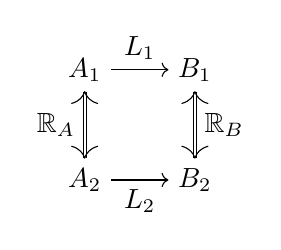
\begin{tikzpicture}[baseline,scale=0.7]
    \node (A1) at (-1,  1) {$A_1$};
    \node (A2) at (-1, -1) {$A_2$};
    \node (B1) at ( 1,  1) {$B_1$};
    \node (B2) at ( 1, -1) {$B_2$};
    \draw (A1) edge[->] node[auto] {$L_1$} (B1);
    \draw (A2) edge[->] node[auto,swap] {$L_2$} (B2);
    \draw (A1) edge[<->, double] node[auto,swap] {$\mathbb{R}_A$} (A2);
    \draw (B1) edge[<->, double] node[auto] {$\mathbb{R}_B$} (B2);
  \end{tikzpicture}
\]

Simulations compose as expected:
we can define the identity simulation convention
$\mathbbm{1}_E : E \Leftrightarrow E$,
which is such that $L \le_{\mathbbm{1}_E \rightarrow \mathbbm{1}_F} L$
for all transition systems $L : E \rightarrow F$,
and define the composite simulation convention
$\mathbb{R} \circ \mathbb{S} : A_1 \Leftrightarrow A_3$ for
$\mathbb{R} : A_1 \Leftrightarrow A_2$ and
$\mathbb{S} : A_2 \Leftrightarrow A_3$,
which describes the type of a composite simulation:
\[
  \AxiomC{$L_1 \le_{\mathbb{R}_A \rightarrow \mathbb{R}_B} L_2$}
  \AxiomC{$L_2 \le_{\mathbb{S}_A \rightarrow \mathbb{S}_B} L_3$}
  \BinaryInfC{$L_1 \le_{\mathbb{R}_A \circ \mathbb{S}_A \rightarrow \mathbb{R}_B \circ \mathbb{S}_B} L_3$}
  \DisplayProof
  \qquad
  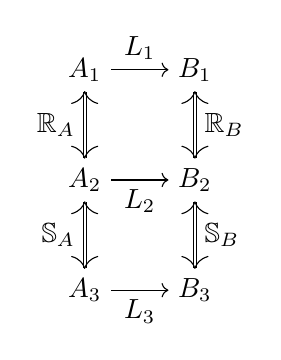
\begin{tikzpicture}[baseline,scale=0.7]
    \node (A1) at (-1,  2) {$A_1$};
    \node (A2) at (-1,  0) {$A_2$};
    \node (A3) at (-1, -2) {$A_3$};
    \node (B1) at ( 1,  2) {$B_1$};
    \node (B2) at ( 1,  0) {$B_2$};
    \node (B3) at ( 1, -2) {$B_3$};
    \draw (A1) edge[->] node[auto] {$L_1$} (B1);
    \draw (A2) edge[->] node[auto,swap] {$L_2$} (B2);
    \draw (A3) edge[->] node[auto,swap] {$L_3$} (B3);
    \draw (A1) edge[<->, double] node[auto,swap] {$\mathbb{R}_A$} (A2);
    \draw (B1) edge[<->, double] node[auto] {$\mathbb{R}_B$} (B2);
    \draw (A2) edge[<->, double] node[auto,swap] {$\mathbb{S}_A$} (A3);
    \draw (B2) edge[<->, double] node[auto] {$\mathbb{S}_B$} (B3);
  \end{tikzpicture}
\]
In addition,
simulation conventions of a given type
are equipped with a notion of refinement $\preceq$,
and for ``endo-conventions'' of type $\mathbb{R} : G \Leftrightarrow G$,
a corresponding notion of Kleene star $\mathbb{R}^*$.

%}}}

\subsubsection{Compiler Correctness} \label{sec:compcert:overview} %{{{

Based on the existing CompCert semantics,
we will define the elementary games
$\mathcal{C}$ and $\mathcal{A}$
describing how C and assembly modules
interact with their respective environments.
The semantics of CompCert $\kw{Clight}$ and $\kw{Asm}$ programs
can then be expressed as interactive behaviors of types:
\[
    \kw{Clight} \llbracket p_s \rrbracket :
      \mathcal{C} \Rightarrow \mathcal{C} \,, \qquad
    \kw{Asm} \llbracket p_t \rrbracket :
      \mathcal{A} \Rightarrow \mathcal{A} \,.
\]
We will show that there exists a simulation convention
$\mathbb{R}_\kw{CompCert} : \mathcal{A} \Leftrightarrow \mathcal{C}$
such that whenever $p_t = \kw{CompCert}(p_s)$,
the following refinement property holds:
\begin{equation}
    \label{eqn:correctness}
    \kw{Asm} \llbracket p_t \rrbracket \,
    \le_{\mathbb{R}_\kw{CompCert} \Rightarrow \mathbb{R}_\kw{CompCert}}
    \kw{Clight} \llbracket p_s \rrbracket
\end{equation}

In Compositional CompCert,
this is achieved independently for each compilation pass.
Stated in our terms,
Compositional CompCert
employs a fixed interface $\mathcal{C}$,
and \emph{structured injections} define a refinement convention
$\mathbb{S} : \mathcal{C} \Leftrightarrow \mathcal{C}$.
A theorem similar to (\ref{eqn:correctness}) is proved for each pass,
and structured injections are shown to compose
($\mathbb{S} \cdot \mathbb{S} \equiv \mathbb{S}$),
so that a theorem can be derived for the whole compiler.

%A major challenge encountered in this context
%is the asymmetry of requirements vs. guarantees
%present in the existing proofs:
%while CompCert imposes strong requirements
%on the semantics of external functions,
%the simulation relations used by its correctness proofs
%are too weak to establish corresponding guarantees
%for a module's own function executions,
%preventing horizontal compositionality.
%Because of this,
%Compositional CompCert required significant changes
%to all compilation passes,
%strengthening their simulation relations
%to conform to $\mathbb{S}$.

Our explicit treatment of abstraction
and reified notion of simulation convention
makes another approach possible.
Using existing proofs, it is straightforward
to establish
for each pass:
\begin{equation}
    \label{correctness-alt}
    \llbracket p_t \rrbracket
    \le_{\mathbb{R} \Rightarrow \mathbb{R}'}
    \llbracket p_s \rrbracket \,,
\end{equation}
where the simulation conventions $\mathbb{R}$ and $\mathbb{R}'$
characterize the assumptions and guarantees
of the existing proof.
In addition,
relevant properties of key source, target, and intermediate languages
can be expressed in relational form,
and can be used to strengthen the resulting theorem:
by composing these proofs together,
and using algebraic properties of
the simulation conventions involved,
we will be able to bridge the gap
between the domain and codomain simulation conventions
and be able to prove a correctness statement
in the form of (\ref{eqn:correctness}),
enabling horizontal compositionality.

%}}}

%}}}

\subsection{Logical relations} %{{{

Logical relations are structure-preserving relations,
in the same way that homomorphisms are structure-preserving maps.
However,
logical relations are more compositional than homomorphisms,
because they do not suffer from the same problems
in the presence of mixed-variance constructions,
such as the function arrow $\rightarrow$ \cite{lrp}.
In the context of typed languages,
this means type-indexed logical relations
can be defined by recursion over the structure of types.

%Logical relations have found widespread use in programming language theory.
%Unary logical relations can be used to establish
%various properties of type systems:
%a type-indexed predicate expressing a property of interest
%is shown to be compatible with the language's reduction,
%and to contain all of the well-typed terms of the language.
%Binary logical relations can be used to capture
%contextual equivalence between terms,
%as well as notions such as non-interference or compiler correctness.
%Relational models of type quantification yield
%Reynold's well-known theory of relational parametricity,
%and can be used to prove \emph{free theorems} that
%all terms of a given parametric type must satisfy.

Logical relations can be of any arity,
but in the present work
we will restrict our attention to
binary logical relations.
Given an algebraic structure $\mathcal{S}$,
a \emph{logical relation}
between two instances $S_1, S_2$ of $\mathcal{S}$
will be a relation $R$
between their carrier sets,
such that the corresponding operations of $S_1$ and $S_2$
take related arguments to related results.
We write $R : \mathcal{R}(S_1, S_2)$.

\begin{example}[Logical relation of monoids]
\label{ex:monoid}
A \emph{monoid} is a set $A$ equipped with
an associative binary operation $\cdot$ and
an identity element $\epsilon$.
A \emph{logical relation of monoids} between
a monoid $\langle A, \cdot_A, \epsilon_A \rangle$ and
a monoid $\langle B, \cdot_B, \epsilon_B \rangle$
is a relation $R \subseteq A \times B$
such that:
\[
(u \ifr{R} u' \wedge v \ifr{R} v' \Rightarrow u \cdot_A v \ifr{R} u' \cdot_B
v')
\: \wedge \:
\epsilon_A \ifr{R} \epsilon_B \,.
\]
\end{example}

Logical relations between multisorted structures
will include one relation for each sort,
between the corresponding carrier sets.
In the case of structures which include type operators,
we can associate to each base type $A$
a relation over its carrier set $\llbracket A \rrbracket$,
and to each type operator $T(A_1, \ldots, A_n)$
a corresponding \emph{relator}:
given relations $R_1, \ldots, R_n$ over
the carrier sets $\llbracket A_1 \rrbracket, \ldots, \llbracket A_n \rrbracket$,
the relator for $T$
will construct a relation $T(R_1, \ldots, R_n)$
over $\llbracket T(A_1, \ldots, A_n) \rrbracket$.

\begin{figure} % fig:relators {{{
  {\small
  \begin{align*}
    x \ifr{R_1 \times R_2} y \ \Leftrightarrow\  &
      \pi_1(x) \ifr{R_1} \pi_1(y) \wedge
      \pi_2(x) \ifr{R_2} \pi_2(y) \\
    x \ifr{R_1 + R_2} y \ \Leftrightarrow\  &
      (\exists \, x_1 \, y_1 \,.\,
        x_1 \ifr{R_1} y_1 \wedge
        x = i_1(x_1) \wedge
        y = i_1(y_1)) \\ \vee\ &
      (\exists \, x_2 \, y_2 \,.\,
        x_2 \ifr{R_2} y_2 \wedge
        x = i_2(x_2) \wedge
        y = i_2(y_2)) \\
    f \ifr{R_1 \rightarrow R_2} g \ \Leftrightarrow\  &
      \forall \, x \, y \,.\,
        x \ifr{R_1} y \Rightarrow
        f(x) \ifr{R_2} g(y) \\
    A \ifr{\mathcal{P}^\le(R)} B \ \Leftrightarrow\  &
      \forall \, x \in A \,.\,
      \exists \, y \in B \,.\,
      x \ifr{R} y
  \end{align*}
  }%
  \caption{A selection of relators}
  \label{fig:relators}
\end{figure}
%}}}

Relators for some common constructions are shown in Fig.~\ref{fig:relators}.
Note that the first requirement given in Example~\ref{ex:monoid} above
can be expressed as
$
  \cdot_A \ifr{R \times R \rightarrow R} \cdot_B
$.

%Logical relations used to reason about contextual equivalence
%are often partial equivalence relations (PER).
%By contrast, since we mainly focus on refinement,
%most of the relations we consider will not be symmetric.

%}}}

\subsection{Kripke logical relations} %{{{
\label{sec:klr}

For stateful languages,
which terms should be related
will often depend on the current state.
Kripke logical relations
are parametrized over a set of state-dependent \emph{worlds}.
Different components related at the same world
will be guaranteed to be related in compatible ways.

In the following,
we give a general account of Kripke logical relations
by drawing on their connection with
the Kripke semantics of modal logic.
We apply this framework
in our treatment of refinement and abstraction
in the context of game semantics (\S\ref{sec:monad:abs}).
Then in \S\ref{sec:compcert:cklr},
we use it to develop a logical-relations
understanding of some key aspects of CompCert,
and show how parametricity
can be used to derive important properties
of CompCert languages.

\begin{definition}
For a set $W$,
a \emph{Kripke logical relation} is
a family of logical relations $(R_w)_{w \in W}$.
We write $R : \mathcal{R}_W(S_1, S_2)$
for a Kripke logical relation between structures $S_1$ and $S_2$,
and define:
\begin{align*}
  x \ifr{w \Vdash R} y &\Leftrightarrow x \ifr{R_w} y \\
  x \ifr{\Vdash R} y &\Leftrightarrow \forall w \,.\, x \ifr{R_w} y \,.
\end{align*}
\end{definition}

\begin{example}[CompCert memory injections] \label{ex:meminj} %{{{
The memory model of CompCert divides the memory into blocks,
whose contents are addressed by an integer
(see \S\ref{sec:compcert:mm}).
Between the states of the source and target programs,
a block may be dropped, added, or
mapped at a given offset within a larger block.
These transformations of the memory structure
are specified by partial functions of type:
\[
  \kw{meminj} := \kw{block} \rightharpoonup \kw{block} \times \mathbb{Z} \,,
\]
The simulation relations of CompCert,
and the component relations that they are built from,
are often parametrized by such a partial function $f : \kw{meminj}$,
which we call an \emph{injection mapping}.
An entry $f(b) = (b', o)$
means that the source memory block with identifier $b$
is mapped into the target memory block with identifier $b'$
at offset $o$.

For example,
CompCert represents pointers as pairs $(b, o)$, where
$b : \kw{block}$ designates a memory block, and
$o : \mathbb{Z}$ specifies an offset within the block.
The correspondance between source and target pointers
depends on the injection mapping being used.
To make sure pointers are related consistently
with each other and with the memory states,
in \S\ref{sec:compcert:mm}
we model this correspondance as a $\kw{meminj}$-indexed
Kripke logical relation $(R^\kw{ptr}_f)_{f : \kw{meminj}}$
defined by:
\[
    (b_1, o_1) \ifr{f \Vdash R^\kw{ptr}} (b_2, o_2) \:\Leftrightarrow\:
    f(b_1) = (b_2, o_2 - o_1) \,.
\]
\end{example}
%}}}

\subsubsection{Kripke relators}

A logical relation $R : \mathcal{R}(A, B)$
can be promoted to a $W$-indexed Kripke logical relation $\lceil R \rceil$
which ignores the index, so that $\lceil R \rceil_w = R$ for all $w \in W$.
Likewise,
a relator
  $F : \mathcal{R}(A_1, B_1) \,\times\,\cdots\,\times\,\mathcal{R}(A_n, B_n) \rightarrow \mathcal{R}(A, B)$
can be promoted to its Kripke version
by pointwise extension over the set of possible worlds:
\begin{gather*}
  \lceil F \rceil : \mathcal{R}_W(A_1, B_1) \times \cdots \times \mathcal{R}_W(A_n, B_n) \rightarrow \mathcal{R}_W(A, B) \\
  \lceil F \rceil (R_1, \ldots, R_n)_w = F(R_{1,w}, \ldots, R_{n,w})
\end{gather*}
We use $\lceil - \rceil$ implicitly
when a relator appears in a context where
a Kripke logical relation is expected.

\subsubsection{Modalities}

Kripke logical relations
can be used to ensure that the components of complex states
are related consistently (at the same world).
By adding structure to the set of worlds,
we will be able to go one step further and
specify how these worlds can evolve,
for instance across time.

\begin{definition} %{{{
A \emph{Kripke frame} is a tuple
$\langle W, {\leadsto} \rangle$, where
$W$ is a set of \emph{possible worlds} and
$\leadsto$ is a
binary \emph{accessibility relation} over $W$.
For a frame
$\langle W, \leadsto \rangle$,
we define the Kripke relators $\Diamond$, $\Box$ as:
\begin{align*}
  x \ifr{w \Vdash \Diamond R} y & \: \Leftrightarrow \:
    \exists \, w' \,.\, w \leadsto w' \wedge
      x \ifr{w' \Vdash R} y \\
  x \ifr{w \Vdash \Box R} y & \: \Leftrightarrow \:
    \forall \, w' \,.\, w \leadsto w' \Rightarrow
      x \ifr{w' \Vdash R} y
\end{align*}
\end{definition}
%}}}

Building on Example~\ref{ex:meminj},
we continue to examine the ways in which
some aspects of CompCert can be understood
in terms of Kripke logical relations.

\begin{example}[CompCert simulation diagrams] \label{ex:sim} %{{{
Many simulation diagrams in CompCert
involve a memory injection.
We can make them more compositional by
expressing them in the framework of Kripke logical relations.
A simulation relation will be a Kripke logical relation
$R \in \mathcal{R}_\kw{meminj}(A, B)$,
which will relate two transition systems
$\alpha : A \rightarrow \mathcal{P}(A)$ and
$\beta : B \rightarrow \mathcal{P}(B)$
according to the diagram:
\[
  \begin{tikzcd}
    s_1 \arrow[r, "\alpha"]
        \arrow[d, dash, "R_f"'] &
    s_1' \arrow[d, dashed, dash, "R_{f'} \quad (f \subseteq f')"] \\
    s_2 \arrow[r, dashed, "\beta"] &
    s_2'
  \end{tikzcd}
\]
More precisely, this diagram represents the following condition:
\[
    \forall f \, s_1 \, s_2 \, s_1' \,.\,
      s_1 \ifr{f \Vdash R} s_2 \wedge
      \alpha(s_1) \ni s_1' \Rightarrow
    \exists f' \, s_2' \,.\,
      \beta(s_2) \ni s_2' \wedge
      f \subseteq f' \wedge
      s_1' \ifr{f' \Vdash R} s_2'
\]
Here, the new states may be related according to
a new memory injection $f'$,
but in order to preserve existing relationships
between source and target pointers,
the new memory injection should include
the original one ($f \subseteq f'$).

This pattern is very common in CompCert
and appears in a variety of contexts.
By using $\langle \kw{meminj}, {\subseteq} \rangle$
as a Kripke frame,
we can express it concisely and compositionally
in our relational framework.
For instance,
using the relator $\mathcal{P}^\le$ defined in
Fig.~\ref{fig:relators},
the simulation diagram shown above can be written as:
\[
  \alpha \ifr{\Vdash R \rightarrow \mathcal{P}^\le(\Diamond R)} \beta \,.
\]
\end{example}
%}}}

%}}}

%}}}

\section{Open Modules for CompCert} \label{sec:compcert} %{{{

\subsection{The CompCert Memory Model} \label{sec:compcert:mm} %{{{

\begin{figure} % fig:mm (The CompCert memory model) {{{
  \footnotesize
  \begin{gather*}
    v : \kw{val} ::=
      \kw{Vundef} \alt
      \kw{Vint}(n) \alt
      \kw{Vlong}(n) \alt
      \kw{Vfloat}(x) \alt
      \kw{Vsingle}(x) \alt
      \kw{Vptr}(b, o)
    \\
    (b, o) : \kw{ptr} :=
      \kw{block} \times \mathbb{Z}
    \\
    (b, l, h) : \kw{ptrrange} :=
      \kw{block} \times \mathbb{Z} \times \mathbb{Z}
  \end{gather*}
  \begin{align*}
    \kw{Mem.alloc} &:
      \kw{mem} \rightarrow \mathbb{Z} \rightarrow \mathbb{Z} \rightarrow
      \kw{mem} \times \kw{block}
    \\
    \kw{Mem.free} &:
      \kw{mem} \rightarrow
      \kw{ptrrange} \rightarrow
      \kw{option}(\kw{mem})
    \\
    \kw{Mem.load} &:
      \kw{mem} \rightarrow \kw{ptr} \rightarrow \kw{option}(\kw{val})
    \\
    \kw{Mem.store} &:
      \kw{mem} \rightarrow \kw{ptr} \rightarrow \kw{val} \rightarrow \kw{option}(\kw{mem})
    \\
    \kw{Mem.perm} &:
      \kw{mem} \rightarrow \kw{ptr} \rightarrow \mathcal{P}(\kw{perm})
  \end{align*}
  \caption{Outline of the CompCert memory model}
  \label{fig:mm}
\end{figure}
%}}}

The CompCert memory model \cite{compcertmmv2}
is the core algebraic structure
which underlies the semantics of CompCert's languages.
Some of its operations
are shown in Fig.~\ref{fig:mm}.
The idealized version presented here
involves
the type of memory states \kw{mem},
the types of pointers \kw{ptr} and address ranges \kw{ptrrange}, and
the type of runtime values \kw{val}.
To keep our exposition concise and clear,
we will gloss over the technical details
associated with the encoding of offsets
as concrete binary integers,
and the associated modular arithmetic and overflow constraints.
[But see artefact for the details.]

The memory is organized into a finite number of \emph{blocks}.
Each memory block has a unique identifier ($b : \kw{block}$)
represented as a positive integer,
and is equipped with its own independent linear address space.
Block identifiers and offsets are often manipulated together,
as a pair $p = (b, o) : \kw{ptr} = \kw{block} \times \mathbb{Z}$.
New blocks are created by the primitive $\kw{Mem.alloc}$,
with prescribed boundaries for their usable offsets.

A runtime value ($v : \kw{val}$) can be stored at
a given address using the primitive \kw{Mem.store},
and retreived using the primitive \kw{Mem.load}.
Values can be integers (\kw{Vint}, \kw{Vlong}) and
floating point numbers (\kw{Vfloat}, \kw{Vsingle})
of different sizes,
as well as pointers (\kw{Vptr}).
The special value \kw{Vundef}
represents an undefined value;
the simulation relations used by CompCert
usually allow $\kw{Vundef}$
to be refined into a more concrete value.

The memory model is shared by all of the languages in CompCert.
The states used to define their semantics consist of
a memory component $m : \kw{mem}$,
together with language-specific components
containing additional run-time values ($\kw{val}$).
For higher-level languages,
the language-specific component may consist of
a control stack with local environments for each activation;
for lower-level languages,
the additional component will mainly contain
the values stored in various registers.

%}}}

\subsection{Language Interfaces} \label{sec:compcert:li} %{{{

\begin{table*} % tbl:li Language interfaces {{{
  \footnotesize
  \begin{tabular}{clll}
    \hline
    Name & Questions & Answers & Description \\
    \hline
    $\mathcal{C}$ & $(\kw{id}, \kw{sg}, \vec{v}, m)$ & $(v', m')$ &
      C-style function calls (Clight--RTL) \\
    $\mathcal{L}$ & $(\kw{id}, \kw{sg}, \kw{ls}, m)$ & $(\kw{ls}', m')$ &
      Arguments passed in abstract locations (LTL, Linear) \\
    $\mathcal{M}$ & $(\kw{id}, \kw{sp},\kw{ra},\kw{rs}, m)$ & $(\kw{rs}', m')$ &
      Arguments passed through in-memory stack (Mach) \\
    $\mathcal{A}$ & $(\kw{rs}, m)$ & $(\kw{rs}', m')$ &
      Assembly-style control transfers (Asm) \\
    \hline
  \end{tabular}
  \caption{Language interfaces for the various languages of CompCert.}
  \label{tbl:li}
\end{table*}
%}}}

The elementary games we use to model
the cross-module interactions of CompCert languages
are shown in Table~\ref{tbl:li}.
Moves correspond to control transfers
between a module and its environment:
questions correspond to function invocations;
answers return control to the caller.

At the source level ($\mathcal{C}$),
questions consist of
the name and signature of the function being invoked,
the values of its arguments,
and the state of the memory at the point of entry;
answers
consist of the function's return value
and the state of the memory at the point of exit.
This language interface is used for Clight and
for the majority of CompCert's intermediate languages.
Once we reach Asm ($\mathcal{A}$),
queries and replies simply specify
the values of registers and the state of the memory.

%}}}

\subsection{Operational Semantics} %{{{
\label{sec:modsem:def}

In the original CompCert,
a labeled transition system is given as
a set of states $S$,
a subset $I \subseteq S$ of initial states,
a labeled transition relation
${\rightarrow} \subseteq S \times \mathbb{E}^* \times S$,
and a set
$F \subseteq S \times \kw{int}$
of final states associated with integer results.
CompCert LTS support a notion of interaction with the environment
in the form of event traces:
a transition $s \stackrel{t}{\rightarrow} s'$,
indicates that the state $s$ may transition to state $s'$
through an interaction recorded as the event trace $t \in \mathbb{E}^*$.
We replace this facility with
an explicit treatment of incoming and outgoing calls
at the level of transition systems.

\begin{definition}[Small-step semantics]
Given two elementary games $A, B$,
a \emph{small-step semantics} for $A \Rightarrow B$
is a tuple $L = \langle S, \rightarrow, I, X, Y, F \rangle$.
${\rightarrow} \subseteq S \times S$ is a \emph{transition relation} on
the set of states $S$.
The handling of incoming calls is specified by
$I \subseteq M_B^\kw{Q} \times S$, which
assigns a set of \emph{initial states} to each question of $B$, and by
$F \subseteq S \times M_B^\kw{A}$,
which designates \emph{final states} together with corresponding answers.
External calls are specified by
$X \subseteq S \times M_A^\kw{Q}$,
which identifies \emph{interacting states} together with
a corresponding question of $A$ directed to the environment, and
$Y \subseteq S \times M_A^\kw{A} \times S$,
which is used to select a \emph{resumption state}
based on the outcome of the external call
after the environment returns.
We write $L : \kw{semantics}(A, B)$ to indicate that
$L$ is a small-step semantics for $A \Rightarrow B$.
\end{definition}

In CompCert, the absence of any transition (``getting stuck'')
denotes an undefined behavior.
This convention fits the context of
language semantics defined through inductive sets of rules:
the behavior of a state for which there are no rules is undefined.
For a small-step semantics
$L = \langle S, {\rightarrow}, I, X, Y, F \rangle : \kw{semantics}(A,B)$,
we recognize those states using the predicate:
\[
    \kw{stuck}_L(s) :=
      ({\rightarrow}(s) = \varnothing) \wedge
      (X(s) = \varnothing) \wedge
      (F(s) = \varnothing)
\]
Taking this into account,
the immediate behavior of a state $s \in S$
can be expressed as the interactive computation
$\kw{step}_L(s) : \mathcal{I}_{M_A^\kw{Q},M_A^\kw{A}}(S)$
defined as follows:
\[
  \kw{step}_L(s) :=
    \begin{cases}
      \top & \mbox{if } \kw{stuck}(s) \\
      {\rightarrow}(s) \sqcup
      (X(s) \bind \mathbf{I} \bind Y(s)) & \mbox{otherwise,}
   \end{cases}
\]
The overall external behavior of $L$
can then be given as
$
    \llbracket L \rrbracket :
      M_B^\kw{Q} \rightarrow \mathcal{I}_{M_A^\kw{Q},M_A^\kw{A}}(M_B^\kw{A})
$
defined by:
%Then $\llbracket L \rrbracket$ can be defined as:
\begin{align*}
  \llbracket L \rrbracket (q) :=
    \begin{cases}
       \top & \mbox{if } I(q) = \varnothing \\
       I(q) \bind \kw{step}^\infty \bind F & \mbox{otherwise.}
     \end{cases}
\end{align*}

%}}}

\subsection{Simulations} \label{sec:modsem:sim} %{{{
\label{sec:modsem:ref}

The correctness of CompCert is established in terms of
\emph{backward simulations}%
\footnote{In this usage, \emph{backward} pertains to
  the compilation process,
  rather than the execution of programs.}
between the small-step semantics of the source and target programs,
which are then shown to be sound with respect to trace containement.
In this section,
we define these notions in our updated context.

A backward simulation asserts that any transition in the target program
has a corresponding transition sequence in the source program.
The source transition sequence may be empty,
but to ensure the preservation of silent divergence
this can only happen for finitely many consecutive target transitions.
This is enforced by indexing the simulation relation
over a well-founded order,
and requiring the index to decrease
whenever an empty source transition sequence is used.

In our setting,
the definition of backward simulations needs to be extended
to take into account the correspondance between
the source and target questions and answers
This can be specified using the following notion.

\begin{definition} % Simulation convention %{{{
A \emph{simulation convention} between the elementary games
$A^\natural = \langle M_{A^\natural}^\kw{Q}, M_{A^\natural}^\kw{A} \rangle$ and
$A^\sharp = \langle M_{A^\sharp}^\kw{Q}, M_{A^\sharp}^\kw{A} \rangle$
is as a tuple $\mathbb{R} = \langle W, R^\kw{Q}, R^\kw{A} \rangle$
with $R^\kw{Q} \in \mathcal{R}_W(M_{A^\natural}^\kw{Q}, M_{A^\sharp}^\kw{Q})$
and $R^\kw{A} \in \mathcal{R}_W(M_{A^\natural}^\kw{A}, M_{A^\sharp}^\kw{A})$.
We will write $\mathbb{R} : A^\natural \Leftrightarrow A^\sharp$.
Given two simulation conventions
$\mathbb{R} : A^\natural \Leftrightarrow A^\sharp$ and
$\mathbb{S} : B^\natural \Leftrightarrow B^\sharp$,
and for two strategies
$\sigma^\natural : A^\natural \Rightarrow B^\natural$ and
$\sigma^\sharp : A^\sharp \Rightarrow B^\sharp$,
we write $\sigma^\natural \le_{\mathbb{R} \Rightarrow \mathbb{S}} \sigma^\sharp$
and say that $\sigma^\natural$ is
\emph{simulated by $\sigma^\sharp$ according to the convention}
$\mathbb{R} \Rightarrow \mathbb{S}$
when the following property holds:
\[
  \sigma^\natural \le_{\mathbb{R} \Rightarrow \mathbb{S}} \sigma^\sharp
  \: := \:
  \sigma^\sharp
  \ifr{\Vdash S^\kw{Q} \rightarrow
       \mathcal{I}_{R^\kw{Q}, R^\kw{A}}(S^\kw{A})}
  \sigma^\natural \,.
\]
\end{definition}
%}}}

defined in \S\ref{sec:monad:abs}:
a simulation between the small-step semantics
$L_1 : \kw{semantics}(A_1, B_1)$ and
$L_2 : \kw{semantics}(A_2, B_2)$ will
operate in the context of the refinement conventions
$\mathbb{C}_A : A_2 \Leftrightarrow A_1$ and
$\mathbb{C}_B : B_2 \Leftrightarrow B_1$.

When relating sets of states,
we will want to make sure that
each \emph{target} state has a corresponding \emph{source} state,
but the source program may allow additional behaviors
that are not realized in the target program.
However, to take into account the convention that
empty sets of states correspond to undefined behaviors,
when the source set is empty,
no restrictions are placed on the target state.

\begin{definition}[Backward simulation between sets of states]
We say that $R : \mathcal{R}(S_1, S_2)$ is a
\emph{backward simulation relation
  between the sets $X_1 \subseteq S_1$ and  $X_2 \subseteq S_2$}
if the following conditions hold:
\begin{enumerate}
\item
  If $X_1$ is non-empty,
  then $X_2$ is non-empty as well.
\item
  If $X_1$ is non-empty,
  then for all $s_2 \in X_2$,
  there exists $s_1 \in X_1$
  such that $(s_1, s_2) \in R$.
\end{enumerate}
We will write $X_1 \ge_R X_2$.
\end{definition}

A state $s$ \emph{goes wrong}
if it is neither an interaction nor a final state,
and if there is no transition $s \rightarrow s'$;
a state $s$ is \emph{safe}
if no state that goes wrong is reachable from $s$
by the transition relation $\rightarrow$.
Safe states will be denoted using the predicate $\kw{safe}(s)$.
We can now define backward simulations.

\begin{definition}[Backward simulation]
Given
$\mathbb{C}_A : A_2 \Leftrightarrow A_1$ and
$\mathbb{C}_B : B_2 \Leftrightarrow B_1$
two simulation conventions,
and given
$L_1 : \kw{semantics}(A_1, B_1)$ and
$L_2 : \kw{semantics}(A_2, B_2)$
two small-step semantics,
a \emph{backward simulation} between $L_1$ and $L_2$
consists in a
well-founded relation $(I, <)$
together with a family of relations
$(R_i : \mathcal{R}_{W_B}(S_1, S_2))_{i \in I}$
satisfying the following properties:
\begin{description}
\item[Initial states]
  For all
  $q_1 \ifr{w \Vdash {\preceq}_B^\kw{Q}} q_2$,
  the condition $I_1(q_1) \ge_{\exists i . R_i} I_2(q_2)$ holds.
\item[Progress]
  For all $s_1 \ifr{w \Vdash R_i} s_2$
  with $s_1$ a safe state,
  $s_2$ does not go wrong.
\item[Simulation]
  For all $s_1 \ifr{w \Vdash R_i} s_2$,
  if $s_1$ is a safe state and $s_2 \rightarrow s_2'$,
  then there exists $i' \in I$ and $s_1' \in S_1$
  such that $s_1' \ifr{w \Vdash R_{i'}} s_2'$ and
  such that 
    $s_1 \rightarrow^+ s_1'$, or
    $s_1 \rightarrow^* s_1' \:\wedge\: i' < i$.
\item[External calls]
  For all $s_1 \ifr{w \Vdash R_i} s_2$
  with $s_1$ a safe state, and
  for any question $m_2 \in M_{A_2}^\kw{Q}$
  such that $(s_2, m_2) \in X_2$,
  there exists $w' \in W_A$ and $q_1 \in M_{A_1}^\kw{Q}$
  such that $q_1 \ifr{w' \Vdash {\preceq}_A^\kw{Q}} q_2$.
  In addition, for all corresponding answers
  $r_1 \ifr{w' \Vdash {\preceq}_A^\kw{A}} r_2$,
  the condition $Y_1(s_1, r_1) \ge_{\exists i . R_i} Y_2(s_2, r_2)$ holds.
\item[Final states]
  For all $s_1 \ifr{w \Vdash R_i} s_2$
  with $s_1$ a safe state, and
  for any answer $r_2 \in M_{B_2}^\kw{A}$
  such that $(s_2, r_2) \in F_2$,
  there exists a state $s_1'$ reachable from $s_1$ and
  an answer $r_1 \in M_{B_1}^\kw{A}$ such that
  $(s_1', r_1) \in F_1$ and $r_1 \ifr{w \Vdash {\preceq}_B^\kw{A}} r_2$.
\end{description}
We will write $L_1 \ge_{\mathbb{C}_A \Rightarrow \mathbb{C}_B} L_2$.
\end{definition}

\begin{definition}[Constructions on simulation conventions] %{{{
Given two simulation conventions
$\mathbb{R}, \mathbb{S} : A^\natural \Leftrightarrow A^\sharp$,
we say that
$\mathbb{R}$ refines $\mathbb{S}$ and write
$\mathbb{R} \preceq \mathbb{S}$
when the following holds for all $w, m_1, m_2$:
\[
      m_1 \ifr{w \Vdash R^\kw{Q}} m_2 \Rightarrow
      \exists \, v \,.\,
        m_1 \ifr{v \Vdash S^\kw{Q}} m_2 \wedge
        \forall \, n_1 \, n_2 \,.\,
          n_1 \ifr{v \Vdash S^\kw{A}} n_2 \Rightarrow
          n_1 \ifr{w \Vdash R^\kw{A}} n_2
\]
The least upper bound of $\mathbb{R}$ and $\mathbb{S}$
is defined as
$
    \mathbb{R} \curlyvee \mathbb{S} :=
      \langle
        W_R + W_S,
        R^\kw{Q} + S^\kw{Q},
        R^\kw{A} + S^\kw{A}
      \rangle
$,
where for $R \in \mathcal{R}_{W_R}(X,Y)$
and $S \in \mathcal{R}_{W_S}(X,Y)$,
the Kripke logical relation $R + S$ is defined as:
\[
    (R + S)_w =
    \begin{cases}
      R_u & \mbox{if } w = i_1(u) \\
      S_v & \mbox{if } w = i_2(v) \,.
    \end{cases}
\]
Given
$\mathbb{R} : A^\flat \Leftrightarrow A^\natural$ and
$\mathbb{S} : A^\natural \Leftrightarrow A^\sharp$,
the composite convention
$\mathbb{R} \cdot \mathbb{S} : A^\flat \Leftrightarrow A^\sharp$ is defined as:
\[
    \mathbb{R} \cdot \mathbb{S} :=
      \langle
        W_R \times W_S, \:
        R^\kw{Q} \cdot S^\kw{Q}, \:
        R^\kw{A} \cdot S^\kw{A}
      \rangle \,.
\]
Finally,
for $\mathbb{R} : A \Leftrightarrow A$,
we define the $n$-fold composition
$\mathbb{R}^n := \mathbb{R} \cdot \mathbb{R} \cdots \mathbb{R}$,
and
$
    \mathbb{R}^* :=
      \bigcurlyvee_{n \in \mathbb{N}} \mathbb{R}^n
$.
\end{definition}
%}}}

\begin{lemma} \label{lemma:kleenesim} %{{{
Consider the strategies
$\sigma^\natural : A^\natural \Rightarrow B^\natural$,
$\sigma^\sharp : A^\sharp \Rightarrow B^\sharp$ and
the refinement conventions
$\mathbb{R}, \mathbb{R}' : A^\natural \Leftrightarrow A^\sharp$ and
$\mathbb{S}, \mathbb{S}' : B^\natural \Leftrightarrow B^\sharp$.
The following properties hold:
\[
  \AxiomC{$\mathbb{R}' \preceq \mathbb{R}$}
  \AxiomC{$\sigma^\natural \le_{\mathbb{R}' \Rightarrow \mathbb{S}'} \sigma^\sharp$}
  \AxiomC{$\mathbb{S} \preceq \mathbb{S}'$}
  \TrinaryInfC{$\sigma^\natural \le_{\mathbb{R} \Rightarrow \mathbb{S}} \sigma^\sharp$}
  \DisplayProof
  \qquad
  \AxiomC{$\sigma^\natural \le_{\mathbb{R} \Rightarrow \mathbb{S}} \sigma^\sharp$}
  \AxiomC{$\sigma^\natural \le_{\mathbb{R} \Rightarrow \mathbb{S}'} \sigma^\sharp$}
  \BinaryInfC{$\sigma^\natural
     \le_{\mathbb{R} \Rightarrow \mathbb{S} \curlyvee \mathbb{S}'} \sigma^\sharp$}
  \DisplayProof
\]
For the strategies
$\sigma^\flat : A^\flat \Rightarrow B^\flat$,
$\sigma^\natural : A^\natural \Rightarrow B^\natural$,
$\sigma^\sharp : A^\sharp \Rightarrow B^\sharp$ and
the refinement conventions
$\mathbb{R} : A^\flat \Leftrightarrow A^\natural$,
$\mathbb{R}' : A^\natural \Leftrightarrow A^\sharp$, and
$\mathbb{S} : B^\flat \Leftrightarrow B^\natural$,
$\mathbb{S}' : B^\natural \Leftrightarrow B^\sharp$,
the following property holds:
\[
  \AxiomC{$\sigma^\flat \le_{\mathbb{R} \Rightarrow \mathbb{S}} \sigma^\natural$}
  \AxiomC{$\sigma^\natural \le_{\mathbb{R}' \Rightarrow \mathbb{S}'} \sigma^\sharp$}
  \BinaryInfC{$\sigma^\flat
    \le_{\mathbb{R} \cdot \mathbb{R}' \Rightarrow \mathbb{S} \cdot \mathbb{S}'}
    \sigma^\sharp$}
  \DisplayProof
\]
Finally,
for
$\sigma, \tau : A \Rightarrow B$
and for
$\mathbb{R} : A \Leftrightarrow A$ and
$\mathbb{S} : B \Leftrightarrow B$,
the following property holds:
\[
  \AxiomC{$\sigma \le_{\mathbb{R} \Rightarrow \mathbb{S}} \tau$}
  \UnaryInfC{$\sigma \le_{\mathbb{R}^* \Rightarrow \mathbb{S}^*} \tau$}
  \DisplayProof
\]
\end{lemma}
%}}}

%}}}

\subsection{Compiler Passes} %{{{

The passes of CompCert fall into three categories
depending on how
the memory states of their source and target languages are related
by their correctness proofs:
\begin{itemize}
\item \emph{Equality} is used when the memory states
  in the source and target execution remain identical,
  for instance when the differences between
  the source and target programs are mostly a matter of syntax,
  but they execute in the same way.
\item \emph{Memory extensions} are somewhat less constrained:
  the target memory is allowed to contain values that are
  \emph{more defined} than that of the source memory,
  and to have less restrictive permissions,
  so that all operations succeeding on the source memory
  will succeed on the target memory as well.
  However,
  the two memory states must share the same overall structure.
\item \emph{Memory injection} relations
  allow the structures of the source and target memories
  to differ, as specified by an injection mapping
  (see Example~\ref{ex:meminj}).
\end{itemize}

Table~\ref{tbl:passes} shows
the intermediate languages and compilation passes
used in our version of CompCert,
together with the respective
language interfaces and
simulation conventions
that are used for each one.
In the remainder of this section,
we will explain how these simulation conventions are constructed
and how the compiler's overall incoming and outgoing conventions
can be reconciled.

\begin{table*} % tbl:passes Passes of Composable CompCert %{{{
  \footnotesize
  \begin{tabular}{lllp{.55\textwidth}}
    \hline
    Language/Pass & Outgoing & Incoming & Description \\
    \hline
    \textbf{Clight} & $\mathcal{C}$ & $\mathcal{C}$ &
      A simpler version of CompCert C;
      expressions have no side-effects. \\
    \emph{Eqn.}~(\ref{eqn:clight}) & $\mathcal{C}[\kw{injp}]^*$ & $\mathcal{C}[\kw{injp}]^*$ &
      \emph{Clight properties} \\
    \kw{SimplLocals} & $\mathcal{C}[\kw{injp}]$ & $\mathcal{C}[\kw{inj}]$ &
      Pulling non-adressable scalar local variables out of memory. \\
    \kw{Cshmgen} & \kw{id} & \kw{id} &
      Simplification of control structures;
      explication of type-dependent computations. \\
    \hline
    \textbf{Csharpminor} & $\mathcal{C}$ & $\mathcal{C}$ &
      Low-level structured language. \\
    \kw{Cminorgen} & $\mathcal{C}[\kw{injp}]$ & $\mathcal{C}[\kw{inj}]$ &
      Stack allocation of local variables whose address is taken. \\
    \hline
    \textbf{Cminor} & $\mathcal{C}$ & $\mathcal{C}$ &
      Low-level structured language,
      with explicit stack allocation of certain local variables. \\
    \kw{Selection} & $\mathcal{C}[\kw{ext}]$ & $\mathcal{C}[\kw{ext}]$ &
      Recognition of operators and addressing modes. \\
    \hline
    \textbf{Cminorsel} & $\mathcal{C}$ & $\mathcal{C}$ &
      Like Cminor, with machine-specific operators and addressing modes. \\
    \kw{RTLgen} & $\mathcal{C}[\kw{ext}]$ & $\mathcal{C}[\kw{ext}]$ &
      Construction of the CFG, 3-address code generation. \\
    \hline
    \textbf{RTL} & $\mathcal{C}$ & $\mathcal{C}$ &
      Register transfer language. \\
    \kw{Tailcall} & $\mathcal{C}[\kw{ext}]$ & $\mathcal{C}[\kw{ext}]$ &
      Recognition of tail calls. \\
    \kw{Renumber} & $\kw{id}$ & $\kw{id}$ &
      Postorder renumbering of the CFG. \\
    \emph{Eqn.}~(\ref{eqn:rtl}) & $\mathcal{C}[\kw{inj}]$ & $\mathcal{C}[\kw{inj}]$ &
      \emph{RTL properties} \\
    \kw{Allocation} & \kw{alloc} & \kw{alloc} &
      Register allocation \\
    \hline
    \textbf{LTL} & $\mathcal{L}$ & $\mathcal{L}$ &
      Location transfer language. \\
    \kw{Linearize} & \kw{id} & \kw{id} &
      Linearization of the CFG \\
    \hline
    \textbf{Linear} & $\mathcal{L}$ & $\mathcal{L}$ &
      Like LTL, but the CFG is replaced by
      a linear list of instructions \\
    \kw{CleanupLabels} & \kw{id} & \kw{id} &
      Removal of unreferenced labels. \\
    \kw{Debugvar} & \kw{id} & \kw{id} &
      Synthesis of debugging information. \\
    \kw{Stacking} & \kw{stacking} & \kw{stacking} &
      Laying out the activation records \\
    \hline
    \textbf{Mach} & $\mathcal{M}$ & $\mathcal{M}$ &
      Like Linear, with a more concrete view of the activation record \\
    \kw{Asmgen} & \kw{asmgen} & \kw{asmgen} &
      Emission of assembly code \\
    \hline
    \textbf{Asm} & $\mathcal{A}$ & $\mathcal{A}$ &
      Assembly language for x86 machines \\
    \hline
  \end{tabular}
  \caption}}

%}}}

\subsection{CompCert Kripke Logical Relations} \label{sec:compcert:cklr} %{{{

Memory extensions and injections
are useful for simulations
because they are specific instances
of logical relations for the CompCert memory model:
they are compatible with memory operations
in the sense that
performing similar operations on related arguments
yields related results.

\subsubsection{Definition} %{{{

We formalize this idea by defining
a notion of Kripke logical relations over the CompCert memory model,
closed under composition, and which
admits memory extensions and injections as particular instances.
As we will see,
more complex relations can also be defined,
and this will make relational parametricity theorems
particularly useful.

\begin{definition}[CompCert Kripke logical relation] \label{def:cklr} %{{{
Consider a tuple $R = (W, \leadsto, f, R^\kw{mem})$,
where
$\langle W, \leadsto \rangle$ is a Kripke frame,
$f : W \rightarrow \kw{meminj}$
associates an injection mapping to each world, and
$R^\kw{mem} : \mathcal{R}_{W}(\kw{mem})$
is a Kripke relation on memory states.
We introduce the Kripke relations
$R^\kw{ptr} : \mathcal{R}_W(\kw{ptr})$ and
$R^\kw{ptrrange} : \mathcal{R}_W(\kw{ptrrange})$
defined by the rules:
\[
  \AxiomC{$f_w(b) = (b', \delta)$}
  \UnaryInfC{$(b, o) \ifr{w \Vdash R^\kw{ptr}} (b', o + \delta)$}
  \DisplayProof
  \qquad
  \AxiomC{$(b_1, l_1) \ifr{w \Vdash R^\kw{ptr}} (b_2, l_2)$}
  \AxiomC{$h_1 - l_1 = h_2 - l_2$}
  \BinaryInfC{$(b_1, l_1, h_1) \ifr{w \Vdash R^\kw{ptrrange}} (b_2, l_2, h_2)$}
  \DisplayProof
\]
and the Kripke relation
$R^\kw{val} : \mathcal{R}_W(\kw{val})$
defined by the rules:
\begin{gather*}
  \forall \, v : \kw{val} \,.\,
    \kw{Vundef} \ifr{\Vdash R^\kw{val}} v \qquad
  \kw{Vptr} : {}
    [\Vdash R^\kw{ptr} \rightarrow R^\kw{val}] \\
  \kw{Vint}, \kw{Vlong}, \kw{Vfloat}, \kw{Vsingle} :
    [\Vdash {=} \rightarrow R^\kw{val}] \,.
\end{gather*}
We say that $R$ is a \emph{CompCert Kripke logical relation}
if the properties shown in Fig.~\ref{fig:cklr-def} are satisfied.
\end{definition}
%}}}

\begin{figure} % fig:cklr-def (Definition of CKLRs) {{{
  \footnotesize
  \begin{gather*}
    {\leadsto} \mbox{ is reflexive and transitive} \\
    f \ifr{(\leadsto) \rightarrow \kw{inject\_incr}} f
  \end{gather*}
  \begin{align*}
      \kw{Mem.alloc} :
        &\Vdash R^\kw{mem} \rightarrow {=} \rightarrow {=} \rightarrow
        \Diamond (R^\kw{mem} \times R^\kw{block})
      \\
      \kw{Mem.free} :
        &\Vdash R^\kw{mem} \rightarrow R^\kw{ptrrange} \rightarrow
        \kw{option}^\le(\Diamond R^\kw{mem})
      \\
      \kw{Mem.load} :
        &\Vdash R^\kw{mem} \rightarrow R^\kw{ptr} \rightarrow
        \kw{option}^\le(R^\kw{val})
      \\
      \kw{Mem.store} :
        &\Vdash R^\kw{mem} \rightarrow R^\kw{ptr} \rightarrow R^\kw{val} \rightarrow
        \kw{option}^\le(\Diamond R^\kw{mem})
      \\
      \kw{Mem.perm} :
        &\Vdash R^\kw{mem} \rightarrow R^\kw{ptr} \rightarrow {\subseteq}
  \end{align*}
  \caption{Axioms for CKLRs}
  \label{fig:cklr-def}
\end{figure}
%}}}

The $R^\kw{mem}$ component is given direcly.
We expect $R^\kw{ptr}$ to be functional
(each source pointer has at most one corresponding target pointer),
and to satisfy the following shift-invariance property:
\[
  \AxiomC{$(b_1, o_1) \ifr{R^\kw{ptr}_w} (b_2, o_2)$}
  \UnaryInfC{$(b_1, o_1 + \delta) \ifr{R^\kw{ptr}_w} (b_2, o_2 + \delta)$}
  \DisplayProof
\]
Any such relation can be uniquely specified by
an injection mapping such as $f$.
We expect the remaining components to be consistent with $R^\kw{ptr}$
and $\kw{Vundef}$ to act as a bottom element for $R^\kw{val}$.
Definition~\ref{def:cklr} follows from these conditions.

Note that $w \Vdash R^\kw{val}$
is equivalent to $\kw{Val.inject}(f_w)$
as defined in CompCert.
Furthermore, the relational property associated to $f$,
together with the definitions of
derived relations such as $R^\kw{ptr}$ and $R^\kw{val}$,
ensure that these relations are monotonic in $w$.
However,
this is not usually the case for $R^\kw{mem}$.

%}}}

\subsubsection{Extensions} %{{{

The simplest CompCert KLR corresponds to memory extensions.
It uses a trivial Kripke frame and injection mapping:
\[
  \kw{ext} :=
    \langle \{*\}, \{(*,*)\}, * \mapsto (b \mapsto b), \kw{Mem.extends} \rangle
\]
Note that $\kw{ext}^\kw{val} = \kw{Val.inject}(b \mapsto b)$
is equivalent to $\kw{Val.lessdef}$,
which is the relation on runtime values that
CompCert uses in conjunction with \kw{Mem.extends}.

%}}}

\subsubsection{Injections} %{{{

In the same vein,
we can reify memory injections as the CompCert KLR:
\[
  \kw{inj} :=
    \langle
      \kw{meminj},
      {\subseteq}, %\kw{inject\_incr},
      f \mapsto f,
      \kw{Mem.inject}
    \rangle
\]
Here the type \kw{meminj} is used directly
as the KLR's worlds.
The accessibility relation $f \subseteq g$
is the inclusion of partial functions,
called $\kw{inject\_incr}$ in CompCert,
which asserts that for all block identifiers $b, b'$ and offsets $\delta$
such that $f(b) = (b', \delta)$,
then $g(b) = (b', \delta)$ as well.

%}}}

\subsubsection{Footprint Preservation} %{{{

Passes which use a memory injection as part of their simulation relation
expect external calls to preserve that injection.
In addition,
external calls are expected to only modify
the parts of the source and target memories
that are within the injection's footprint:
addresses that are
related by the injection mapping,
and are granted non-empty permissions
in both memory states.

For instance,
in the \kw{Stacking} pass,
the target memory's stack frames
are extended with spilling locations.
These locations are used in the target program
to keep track of temporary values,
which in the source program are kept
in a local environment separate from the memory state.
The spilling locations are not part of
the injection footprint
because they are unallocated in the source memory;
their preservation across external calls
is essential to the correctness of \kw{Stacking}.

This expectation is reasonable because
external calls
should behave uniformly between the source and target executions.
In particular,
an external function acting on the memory state
should not synthesize block identifiers and pointers,
but can only follow pointers passed as arguments
or fetched from the memory itself.
If it were to access a spilling location in this way in the target execution,
the corresponding source pointer would have to be
related to the target pointer by \kw{Val.inject},
and consequently would either be undefined
or invalid (point to a location without permissions),
so that the source program would go wrong.

Because the CKLR framework is rich enough to express
temporal properties such as the preservation of injection footprints,
this argument can be made precise as a \emph{parametricity} property
(\S\ref{sec:compcert:param}).
For now,
we show how to encode this requirement as a CKLR.

\begin{definition}
The components of the CompCert Kripke logical relation:
\[ \kw{injp} :=
  \langle
    W \times \kw{mem} \times \kw{mem},
    \leadsto_\kw{injp}, \pi_1, R_\kw{injp}^\kw{mem}
  \rangle \]
are defined as follows.
For the injection mappings $f, f'$ and
the memory states $m_1, m_2, m_1', m_2'$,
the relation $(f, m_1, m_2) \leadsto_\kw{injp} (f', m_1', m_2')$
holds when the following conditions are satisfied:
\begin{itemize}
\item $f \subseteq f'$, and any new mappings in $f'$
  must be between newly allocated blocks in $m_1'$ and $m_2'$;
\item any blocks of $m_1$ unmapped by $f$
  must remain unchanged in $m_2$;
\item any locations in $m_2$ unrelated by $f$
  to valid locations of $m_1$ must remain unchanged in $m_2'$;
\item within allocated blocks of $m_1$,
  the permissions assigned to any offset may not increase in $m_1'$
  (this helps ensure that $\leadsto_\kw{meminj}$ is transitive).
\end{itemize}
The relation $R_\kw{injp}^\kw{mem}$ is defined by the rule:
\[
  \AxiomC{$m_1 \ifr{f \Vdash \kw{Mem.inject}} m_2$}
  \UnaryInfC{$m_1 \ifr{(f, m_1, m_2) \Vdash R_\kw{injp}^\kw{mem}} m_2$}
  \DisplayProof
\]
\end{definition}

%}}}

\subsubsection{Relational Parametricity} \label{sec:compcert:param} %{{{

For each language interface
$\mathcal{X} \in \{ \mathcal{C}, \mathcal{L}, \mathcal{M}, \mathcal{A} \}$,
a CKLR
$R = \langle W, {\leadsto}, f, R^\kw{mem} \rangle$ can be promoted to
a simulation convention
$\mathcal{X}[R] : \mathcal{X} \Leftrightarrow \mathcal{X}$.
For example
we define $\mathcal{C}[R] : \mathcal{C} \Leftrightarrow \mathcal{C}$
as follows:
\[
    \mathcal{C}[R] := \langle
      W, \:
      ({=} \times {=} \times {R^\kw{val}}^* \times R^\kw{mem}), \:
      \Diamond (R^\kw{val} \times R^\kw{mem})
    \rangle \,.
\]
Such operators preserve composition
in the sense that $\mathcal{X}[R ; S] = \mathcal{X}[R] \cdot \mathcal{X}[S]$.

Because the semantics of CompCert languages
are expected to be well-behaved with respect to
invariance properties of the memory model,
we can prove for each language of CompCert
a parametricity theorem of the form
$
    \forall R \,.\,
      \llbracket p \rrbracket
        \le_{\mathcal{X}[R] \Rightarrow \mathcal{X}[R]}
      \llbracket p \rrbracket
$.
Since both sides of the relation are identical,
the simulations can be iterated
to obtain similar properties in terms of $\mathcal{X}[R]^*$.

In particular,
we use this approach to establish the following properties,
which will be useful to derive our final correctness theorem:
\begin{gather}
    \forall R \,.\,
      \kw{Clight} \llbracket p \rrbracket
        \le_{\mathcal{C}[R]^* \Rightarrow \mathcal{C}[R]^*}
      \kw{Clight} \llbracket p \rrbracket
      \label{eqn:clight}
      \\
    \forall R \,.\,
      \kw{RTL} \llbracket p \rrbracket
        \le_{\mathcal{C}[R] \Rightarrow \mathcal{C}[R]}
      \kw{RTL} \llbracket p \rrbracket
      \label{eqn:rtl}
\end{gather}
In addition,
the CKLRs defined above satisfy the following
composition properties:
\[
  \mathcal{C}[\kw{inj}] \cdot \mathcal{C}[\kw{inj}] \equiv
  \mathcal{C}[\kw{ext}] \cdot \mathcal{C}[\kw{inj}] \equiv
  \mathcal{C}[\kw{inj}] \cdot \mathcal{C}[\kw{ext}] \equiv
  \mathcal{C}[\kw{inj}] \,.
\]

%}}}

%}}}

\subsection{Compiler Correctness} %{{{

Following the approach outlined in \S\ref{sec:compcert:overview},
and referring to Table~\ref{tbl:passes},
the overall simulation convention for the whole compiler
can be given as:
\[
  \mathbb{R}_\kw{CompCert} : \mathcal{C} \Leftrightarrow \mathcal{A} :=
    \mathcal{C}[\kw{injp}]^* \cdot
    \mathcal{C}[\kw{inj}] \cdot
    \kw{alloc} \cdot
    \kw{stacking} \cdot
    \kw{asmgen} \,.
\]
To verify that the passes indeed compose to
establish correctness with respect to the simulation convention
$\mathbb{R}_\kw{CompCert} \Rightarrow \mathbb{R}_\kw{CompCert}$,
it suffices to show that
the incoming and outgoing simulations can be reconciled,
or more precisely:
\[
    \mathcal{C}[\kw{injp}]^* \cdot
    \mathcal{C}[\kw{injp}] \cdots
    \mathcal{C}[\kw{ext}] \cdot
    \mathcal{C}[\kw{inj}]
    \: \preceq \:
    \mathbb{R}_\kw{CompCert}
    \: \preceq \:
    \mathcal{C}[\kw{injp}]^* \cdot
    \mathcal{C}[\kw{inj}] \cdots
    \mathcal{C}[\kw{ext}] \cdot
    \mathcal{C}[\kw{inj}] 
\]
This follows from the properties outlined above,
so that we can conclude:
\[
    \forall p_s \,.\,
      \kw{CompCert}(p_s) = p_t \Rightarrow
      \kw{Clight} \llbracket p_s \rrbracket
      \le_{\mathbb{R}_\kw{CompCert} \Rightarrow \mathbb{R}_\kw{CompCert}}
      \kw{Asm} \llbracket p_t \rrbracket \,.
\]

%}}}

%}}}

\section{Refinement-Based Game Semantics} \label{sec:monad} %{{{

\subsection{Overview} %{{{

As a first step towards
the development of refinement-based game semantics,
we present a semantic framework
integrating refinement and abstraction
into a simple game model.
To facilitate the expression of operational constructions
within this framework,
we formulate our model around an \emph{interaction monad},
which generalizes strategies to enable
sequential composition and iteration.

\subsubsection{Games} %{{{

We will consider the alternating, well-bracketed, receptive strategies
for the game $!A \multimap B$ (see \S\ref{sec:mainideas:gs:comp})
where $A$ and $B$ are games with a very simple structure.

\begin{definition} \label{def:elemgame} % elementary game {{{
An \emph{elementary game} is a pair
$A = \langle M_A^\kw{Q}, M_A^\kw{A} \rangle$, where
$M_A^\kw{Q}$ is a set of \emph{questions}, and
$M_A^\kw{A}$ is a set of \emph{answers}.
\end{definition}
%}}}

Elementary games proceed as follows:
first $\kw{O}$ chooses a question,
then $\kw{P}$ chooses an answer.
More interestingly,
the composite game $!A \multimap B$
consists of
an instance of $B$, played concurrently with
instances of $A$ in which the roles of $\kw{P}$ and $\kw{O}$ are exchanged.
Hence,
the opponent moves are
$M^\kw{O}_{!A \multimap B} = M^\kw{Q}_B + M^\kw{A}_A$,
the proponent moves are
$M^\kw{P}_{!A \multimap B} = M^\kw{A}_B + M^\kw{Q}_A$,
and alternating, well-bracketed plays
proceed as follows:
\begin{itemize}
  \item The environment first plays a question from the set $M_B^\kw{Q}$.
  \item The system may then ask a question from $M_A^\kw{Q}$,
    which will be answered by the environment with a move in $M_A^\kw{A}$.
    This can be iterated any number of times, at the system's discretion.
  \item The system then plays a move from $M_B^\kw{A}$
    to answer the environment's original question.
\end{itemize}
%\[
%  \begin{tikzpicture}[baseline=(O.base)]
%    \node (I) at (0,0) {};
%    \node (P) at (1,0) {\kw{P}};
%    \node (O) at (2,0) {\kw{O}};
%    \path [->] (I) edge[bend left] node[auto] {$m$} (P);
%    \path [->] (P) edge[bend left] node[auto] {$n$} (O);
%    \path [->] (P) edge[bend left] node[auto] {$q$} (I);
%    \path [->] (O) edge[bend left] node[auto] {$r$} (P);
%  \end{tikzpicture}
%  \quad
%  \begin{array}{c@{\,}l@{\quad}c@{\,}l}
%    m &\in M_B^\kw{Q} & q &\in M_A^\kw{Q} \\[1ex]
%    n &\in M_B^\kw{A} & r &\in M_A^\kw{A}
%  \end{array}
%\]

%}}}

\subsubsection{Strategies} %{{{

Following the usual approach,
we will represent strategies as prefix-closed sets of alternating plays.
Because we limit ourselves to receptive strategies,
odd-length plays can remain implicit and be left out of the representation.
Taking well-bracketing into account,
a first approximation of the type of strategies
for the game $!A \multimap B$ is:
\[
  \mathcal{S}_{!A \multimap B} \: \approx \:
   \big\{ \sigma \subseteq
      M^\kw{Q}_B
      \big( M^\kw{Q}_A M^\kw{A}_A \big)^*
      \big( M^\kw{Q}_A \cup M^\kw{A}_B \big) \: \big| \:
      \sigma \mbox{ prefix-closed} \big\}
\]

%}}}

\subsubsection{Composition} \label{sec:sem:games:comp} %{{{

Consider two strategies
$\sigma : \mathcal{S}_{!A \multimap B}$ and
$\tau : \mathcal{S}_{!B \multimap C}$.
In the composite strategy
$\tau \circ \sigma : \mathcal{S}_{!A \multimap C}$,
$\sigma$ and $\tau$ interact
with each other over their common game $B$,
and with the environment over the respective games $A$ and $C$.
Because $\tau$ may invoke $\sigma$ multiple times,
we need to first promote $\sigma$ to a strategy
$\sigma^\dagger : \mathcal{S}_{{!A} \multimap {!B}}$,
which duplicates the behavior of $\sigma$ to answer several independent questions.
Writing $s \restriction X,Y$ for
the subsequence of $s$ consisting of the moves played in the games $X$ or $Y$,
the traditional formulation of composition
can be given as:
\[
    \tau \circ \sigma =
    \{ s \restriction {A,C} \mid
       s \restriction {A,B} \in \sigma^\dagger \wedge
       s \restriction {B,C} \in \tau \} \,.
\]

Composition may turn two reactive strategies
into a strategy exhibiting silent divergence.
This will happen when
the two strategies only interact over the middle game ($s \in B^*$).
Since in this case $s \restriction A,C$ will be empty,
the formulation given above is appropriate when
silent divergence is identified with the empty interaction.
However,
in the presence of nondeterminism,
this representation of divergence is insufficient \cite{gsnondet}.
In \S\ref{sec:monad:int}
we present an alternative
account of strategy composition.

%}}}

\subsubsection{Nondeterminism} %{{{

Since we wish to model specifications
allowing a range of possible concrete behaviors,
we do not impose
the usual determinism requirement on strategies.
At any given point,
a strategy may allow several possible behaviors
of the system, or none,
and we will use trace containement as
the corresponding notion of refinement.
The introduction of nondeterminisim raises the question of
where divergence fits with respect to that refinement preorder.

%}}}

\subsubsection{Divergence} %{{{

Identifying silent divergence with $\bot$
would allow a diverging program to refine any specification.
Instead,
we wish to treat divergence as a behavior on par with others.
This means our model must be extended
with an explicit representation of silent divergence.
In \cite{gsnondet},
this is accomplished by adjoining to every strategy
a set of the plays which may diverge.
Equivalently,
we extend our model by allowing plays to
signal divergence using
the special move $\Delta$.

%Note that by contrast with \cite{gsnondet},
%[b/c monad gives us just enough branching-time info,
%we don't run into problems with unbounded nondeterminism]

%}}}

\subsubsection{Abstraction} %{{{

We consider forms of abstractions where
the abstract and concrete interactions have the same structure,
but use different representations for their questions and answers.
The correspondance is specified
using Kripke logical relations,
so that we can ensure that questions and answers are related consistently.
Once a concretization relation has been specified
for the constituent games,
this can be extended to a concretization embedding for strategies.
See \S\ref{sec:monad:abs}.

%}}}

\subsubsection{Undefined Behaviors} %{{{

As discussed in \S\ref{sec:mainideas:gs:ref},
we will sometimes want to express undefined behaviors:
specifications which place no restriction on
the actual behavior of the system.
Such specifications could simply be expressed
as a nondeterministic choice between all possible defined behaviors,
however in the presence of abstraction this is unsatisfactory.

Specifically,
the concretization of undefined behaviors
should itself be fully undefined,
but the naive approach would only yield
a nondeterminic choice between all defined concrete behaviors
\emph{for which there is a corresponding abstract behavior}.
To avoid such issues,
we introduce a distinguished representation for undefined behaviors,
in the form of the special move $\lightning$.

%}}}

\subsubsection{Sequential Compositionality} %{{{

Finally,
we generalize from strategies to
define the \emph{interaction monad} $\mathcal{I}_{M,N}(-)$
so that the well-bracketed strategies for $!A \multimap B$
correspond to the special case:
\[
    \mathcal{S}_{!A \multimap B} \: \approx \:
    M_B^\kw{Q} \rightarrow \mathcal{I}_{M_A^\kw{Q},M_A^\kw{A}}(M_B^\kw{A}) \,.
\]
A computation $x \in \mathcal{I}_{M,N}(X)$ in this monad
specifies the behavior of an open system,
which may at any point perform an output $m \in M$ and
wait for a subsequent input $n \in N$ from the environment.
This is modelled by the operation
$\mathbf{I} : M \rightarrow \mathcal{I}_{M,N}(N)$.

%Additionally,
%to accomodate specifications which permit a range of possible behaviors,
%the interaction monad is equipped with a complete refinement lattice.
%Given $x, y : \mathcal{I}_{M,N}(A)$,
%their supremum $x \sqcup y : \mathcal{I}_{M,N}(A)$
%is the smallest specification that permits the behavior of either;
%it can also be interpreted as non-deterministic choice
%of the system.
%Conversely, $x \sqcap y : \mathcal{I}_{M,N}(A)$ can be interpreted as
%the largest specification requiring that $x$ and $y$ both be satisfied.
%The least element $\bot$
%is a specification that can never be satisfied;
%the greatest element $\top$
%is the specification that is always satisfied ---
%or represents a computation whose behavior is entierely undefined.
%
%Finally,
%we model non-deterministic iteration with the operator:
%\[
%     -^\infty : (A \rightarrow \mathcal{I}_{M,N}(A)) \rightarrow
%                (A \rightarrow \mathcal{I}_{M,N}(A)) \,.
%\]
%Notably,
%$-^\infty$ is different from
%the Kleene star associated with the refinement lattice,
%because we account for silent divergence as a specific behavior,
%incomparable with terminating ones,
%rather than identifying it with
%the unsatisfiable specification $\bot$
%or the undefined behavior $\top$.

%}}}

\begin{figure} % fig:notations {{{
  \begin{center}
    \begin{tabular}{lccccccc}
      \hline
      Category & Appl. & Comp. & Unit & Join & Zero & Iteration \\
      \hline
      Functions & $f(x)$ & $f \circ g$ & \kw{id} & & \\
      Monad &
        $x \bind f$ & $g \cdot f$ & $\kw{ret}, \mathbf{1}$ &
        ${\sqcup}, {\oplus}$ & $\bot, \mathbf{0}$ & ${*}, {\infty}$ \\
      Interaction &
        $x[f]$ & $g \odot f$ & $\mathbf{I}$ &
        ${\sqcup}, {\oplus}$ & $\bot, \mathbf{0}$ & $\circledcirc$ \\
      \hline
    \end{tabular}
  \end{center}
  \caption{Summary of notations}
  \label{fig:notations}
\end{figure}
%}}}

%[the monadic approach gives us just enough
%local/intermediate branching-time info
%that we can avoid the usual problems
%around unbounded nondeterminism.]

%}}}

\subsection{The Interaction Monad} \label{sec:monad:def} %{{{

We now formally define the monad $\mathcal{I}_{M,N}$,
starting with the representation of plays. 
Note that
in an interactive behavior
$x \in \mathcal{I}_{M,N}(X)$,
the system is active first,
and may return control to the environment
by performing an output.
The plays we will consider for $\mathcal{I}_{M,N}(X)$
therefore start with a move $m \in M$ of player $\kw{P}$
and be of odd length,
and we use Kleisli morphisms
($f : A \rightarrow \mathcal{I}_{M,N}(B)$)
to encode strategies
which expect $\kw{O}$ to play first.

To support the monadic structure and account
for silent divergence and undefined behaviors,
we augment the set $M$ of outputs with the
distinguished terminal moves
$v \in X$ (returned value),
$\Delta$ (silent divergence), and
$\lightning$ (undefined behavior):
\[
    s, t \in
    \mathcal{T}_{M,N}(X) ::=
    v \mid \Delta \mid \lightning \mid m \mid mnt \,.
\]
Any trace refines $\lightning$, so that
the extended prefix relation on $\mathcal{T}_{M,N}(X)$
is defined by the rules:
\begin{gather*}
  v \sqsubseteq v , \quad
  \Delta \sqsubseteq \Delta , \quad
  t \sqsubseteq \lightning , \quad
  m \sqsubseteq m , \quad
  m \sqsubseteq mnt ,
  \quad
  \AxiomC{$s \sqsubseteq t$}
  \UnaryInfC{$mns \sqsubseteq mnt$}
  \DisplayProof
\end{gather*}
An interactive behavior is
a prefix-closed set of traces:
\[
    \mathcal{I}_{M,N}(X) :=
    \{ T \subseteq \mathcal{T}_{M,N}(X) \mid
       \forall t \in T \,.\, \forall s \sqsubseteq t \,.\, s \in T \}
\]

Note that since any trace is a prefix of $\lightning$,
a behavior which admits a trace ending with $\lightning$
will also admit all possible interactions
sharing the same initial segment.
This allows us to define our notion of refinement
as simple trace containment.
For $x, y \in \mathcal{I}_{M,N}(X)$, refinement is defined as:
\[
    x \sqsubseteq y \Leftrightarrow x \subseteq y
\]
Since unions and intersections
preserve prefix closure,
they induce a lattice structure on $\mathcal{I}_{M,N}(X)$.

%}}}

\subsection{Monad operations} %{{{

The monad's unit associates to each value $v \in X$
the interactive behavior with a single trace $v$:
\[
    \kw{ret}_X(v) := \{ v \} \,.
\]
The binding operation corresponds to
the sequential composition of
a behavior $x \in \mathcal{I}_{M,N}(A)$ and
a Kleisli morphism $f : A \rightarrow \mathcal{I}_{M,N}(B)$.
The result is an interactive behavior
$(x \bind f) \in \mathcal{I}_{M,N}(B)$
containing the traces of $x$ where
any final value $v$ has been replaced with
all possible traces in $f(v)$.
For a single trace $t \in x$ we define $t \bind f$
using the following rules:
\begin{gather*}
  \Delta \in (\Delta \bind f)
  \qquad
  t \in (\lightning \bind f)
  \qquad
  m \in (m \bind f)
  \\[1ex]
  \AxiomC{$t \in f(v)$}
  \UnaryInfC{$t \in (v \bind f)$}
  \DisplayProof
  \quad
  \AxiomC{$s \in (t \bind f)$}
  \UnaryInfC{$mns \in (mnt \bind f)$}
  \DisplayProof
\end{gather*}
Then $x \bind f$ can be defined as:
\[
    (x \bind f) = \bigcup_{t \in x} (t \bind f)
\]
It is straightforward to verify that
the monad laws hold:
\begin{align*}
  (\kw{ret}(v) \bind f) &= f(v) \\
  (x \bind \kw{ret}) &= x \\
  (x \bind (v \mapsto f(v) \bind g)) &= ((x \bind f) \bind g) \,.
\end{align*}

The binding operation $\bind$
and the lattice on $\mathcal{I}_{M,N}(A)$
can be extended to Kleisli morphisms:
\begin{align*}
    (f \cdot g)(a) &:= f(a) \bind g &
    \mathbf{1}(a) &:= \kw{ret}(a) \\
    (f \oplus g)(a) &:= f(a) \sqcup g(a) &
    \mathbf{0}(a) &:= \bot
\end{align*}
Together with the iteration principles
defined in the following section,
these operations constitute a structure
analogous to a typed Kleene algebra \cite{tka}.

%}}}

\subsection{Iteration} \label{sec:monad:iter} %{{{

% TODO: use f^\omega = f^* f_\Delta presentation

A Kleisli morphism $f : A \rightarrow \mathcal{I}_{M,N}(A)$
can be iterated as follows.
We define
$f^n, f^* : A \rightarrow \mathcal{I}_{M,N}(A)$,
respectively the $n$-fold sequential composition of $f$
and the associated notion of Kleene star, as:
\[
  \begin{array}{rl}
    f^0(a) &:= \kw{ret}(a) \\
    f^{n+1}(a) &:= f^n(a) \bind f
  \end{array}
  \qquad
  f^*(a) := \bigsqcup_n f^n(a) \,.
\]
In order to recognize silent divergence,
we introduce $f_\Delta$,
defined by the following coinductive rule.
\[
    \AxiomC{$v' \in f(v)$}
    \AxiomC{$\Delta \in f_\Delta(v')$}
    \doubleLine
    \BinaryInfC{$\Delta \in f_\Delta(v)$}
    \DisplayProof
\]
Note that $f_\Delta(v) \sqsubseteq \{\Delta\}$.
The nondeterministic, infinite iteration of $f$ is
$f^\infty := (f \oplus f_\Delta)^*$.

%}}}

\subsection{Sets and Functions} \label{sec:monad:powerset} %{{{

The powerset monad $\mathcal{P}$
can be embedded into the monad $\mathcal{I}_{M,N}$
through the natural transformation
$\eta^\mathcal{P}_X : \mathcal{P}(X) \rightarrow \mathcal{I}_{M,N}(X)$
defined as
$\eta^\mathcal{P}_X(V) := \{ v \mid v \in V \}$.
In particular,
a relation $R : A \rightarrow \mathcal{P}(B)$
can be interpreted as
$\eta^\mathcal{P}_B \circ R : A \rightarrow \mathcal{I}_{M,N}(B)$.

\begin{example} \label{ex:ts} % Transition system {{{
Consider a transition system $\alpha = (S, I, {\rightarrow}, F)$,
where
$S$ is a set of states,
$I \in \mathcal{P}(S)$
is a set of initial states,
${\rightarrow} : S \rightarrow \mathcal{P}(S)$
is a transition relation, and
$F : S \rightarrow \mathcal{P}(A)$
associates potential output values to each state.
The behavior of $\alpha$ can be expressed as:
\[
    \llbracket \alpha \rrbracket :=
    \eta^\mathcal{P}_S(I) \bind
    (\eta^\mathcal{P}_S \circ {\rightarrow})^\infty \bind
    (\eta^\mathcal{P}_S \circ F)
    : \mathcal{I}_{M,N}(A) \,.
\]
\end{example}
%}}}

We use a similar approach in \S\ref{sec:modsem:def}
to express the behavior of CompCert small-step semantics
in terms of interactive behaviors.
For conciseness,
we will sometimes rely implicitly on $\eta_X^\mathcal{P}$
when a set $x \in \mathcal{P}(A)$ is used
in a context where an interactive behavior
of type $\mathcal{I}_{M,N}(A)$ is expected,
for instance expressing $\llbracket \alpha \rrbracket$ above as
$I \bind {\rightarrow}^\infty \bind F$.

For $f : A \rightarrow B$,
its \emph{preimage}
$f^{-1} : B \rightarrow \mathcal{I}_{M,N}(A)$
can be defined as
$f^{-1}(b) = \eta^\mathcal{P}_A(\{ a \mid f(a) = b \})$.
For instance, given
$f : A \rightarrow \mathcal{I}_{M,N}(X)$ and
$g : B \rightarrow \mathcal{I}_{M,N}(X)$,
their copairing $[f, g] : A + B \rightarrow \mathcal{I}_{M,N}(X)$
in the Kleisli category can be expressed as
$(i_1^{-1} \cdot f) \oplus (i_2^{-1} \cdot g)$.
For the sake of symmetry we will sometimes implicitly promote
$f : A \rightarrow B$ to the Kleisli morphism
$\kw{ret} \circ f : A \rightarrow \mathcal{I}_{M,N}(B)$.

%}}}

\subsection{Interaction} \label{sec:monad:int} %{{{

The interaction primitive
$\mathbf{I}_{M,N} : M \rightarrow \mathcal{I}_{M,N}(N)$
can be defined as
$
    \mathbf{I}_{M,N}(m) := \{ m, mnn \mid n \in N \}
$.
Note that in the trace $mnn$,
the first occurence of $n$ denotes an input,
whereas the second one denotes the value returned by $\mathbf{I}$.

Interaction introduces a second notion of composition
besides the one induced by the $\bind$ operator:
given
$x \in \mathcal{I}_{M,N}(A)$ and
$f : M \rightarrow \mathcal{I}_{P,Q}(N)$,
the behavior $x[f] : \mathcal{I}_{P,Q}(A)$
will proceed according to $x$,
but whenever $x$ attempts to perform an output $m \in M$,
the behavior $f(m)$ will be substituted;
if $f(m)$ returns a value $n \in N$,
the value will be used as an input to resume to evaluation of $x$.
This corresponds to the composition of strategies
discussed in \S\ref{sec:mainideas:gs:comp}.

To formally define the behavior $x[f]$,
we first introduce the following decomposition of $x$:
\[
    x \: = \: \rho(x) \: \sqcup \:
        (\mu(x) \bind m \mapsto \mathbf{I}(m) \bind n \mapsto \delta_{mn}(x))
\]
The residual $\rho(x)$
contains the traces of $x$ that are of the form $v$, $\Delta$ or $\lightning$
(closed under the prefix relation as appropriate).
The behavior $\mu(x)$ contains the traces of $x$ of the form $m$.
The derivative $\delta_{mn}(x)$ is defined as
$\delta_{mn}(x) := \{ t \mid mnt \in x \}$.
Substitution can then be defined as follows.

\begin{definition}[Substitution]
For
$x \in \mathcal{I}_{M,N}(A)$ and
$f : M \rightarrow \mathcal{I}_{P,Q}(N)$,
we define the interactive substitution
$x[f] \in \mathcal{I}_{P,Q}(A)$ as:
\[
    x[f] \: :=
      (s \mapsto \mu(s) \bind
       m \mapsto f(m) \bind
       n \mapsto \kw{ret}(\delta_{mn}(s)))^\infty(x) \bind
      \rho \,.
\]
Additionally, for
$g : A \rightarrow \mathcal{I}_{M,N}(B)$,
the interactive composition
is $(g \odot f)(a) := g(a)[f]$.
\end{definition}

The definition above uses a transition system
over states $s \in \mathcal{I}_{M,N}(A)$.
At any point,
$x[f]$ exhibits the immediate behavior $\rho(s)$.
If $s$ attempts to interact with an output $m$,
$x[f]$ will exhibit the behavior $f(m)$ instead,
and continue whenever $f$ returns $n$
in the next state $\delta_{mn}(s)$.

The interactive substitution and composition
enjoy the following properties:
\begin{align*}
  x[\mathbf{I}] &= x &
  \mathbf{I}(m)[f] &= f(m) &
  x[g \odot f] &= x[g][f] \\
  g \odot \mathbf{I} &= g &
  \mathbf{I} \odot f &= f &
  h \odot (g \odot f) &= (h \odot g) \odot f
\end{align*}

%}}}

\subsection{Abstraction} \label{sec:monad:abs} %{{{

We now consider the problem of relating interactive behaviors
whose inputs, outputs, and results are taken in different sets.
Specifically,
for a \emph{concrete} behavior
$x^\natural : \mathcal{I}_{M^\natural,N^\natural}(X^\natural)$
on one hand, and an \emph{abstract} behavior
$x^\sharp : \mathcal{I}_{M^\sharp,N^\sharp}(X^\sharp)$
on the other hand,
we wish to describe the correspondance between
the two interactions
and establish that
$x^\natural$ is indeed a sound realization of $x^\sharp$.

We use Kripke logical relations to ensure that
outputs are related consistently with their subsequent inputs.
For
a relation $R_M : \mathcal{R}_W(M^\natural, M^\sharp)$ on outputs,
a relation $R_N : \mathcal{R}_W(N^\natural, N^\sharp)$ on inputs,
and a relation $R_X : \mathcal{R}(X^\natural, X^\sharp)$ on results,
our goal will be to define a relator:
\[ \mathcal{I}^\le_{R_M,R_N}(R_X) \: : \:
   \mathcal{R}(\mathcal{I}_{M^\natural,N^\natural}(X^\natural),
               \mathcal{I}_{M^\sharp,N^\sharp}(X^\sharp)) \]
such that $x^\natural \ifr{\mathcal{I}^\le_{R_M,R_N}(R_X)} x^\sharp$
whenever $x^\natural$ is simulated by $x^\sharp$ according to
the correspondance specified by $R_M$, $R_N$ and $R_X$.
We will proceed by defining a concretization mapping:
\[ \gamma_{R_M,R_N,R_X} : \mathcal{I}_{M^\sharp,N^\sharp}(X^\sharp) \rightarrow
                    \mathcal{I}_{M^\natural,N^\natural}(X^\natural) \, \]
such that $\gamma_{R_M, R_N, R_X}(x^\sharp)$ is
the largest computation in $\mathcal{I}_{M^\natural,N^\natural}(X^\natural)$
simulated by $x^\sharp$.
Accordingly,
\[ x^\natural \ifr{\mathcal{I}^\le_{R_M,R_N}(R_X)} x^\sharp
   \: \Leftrightarrow \:
   x^\natural \sqsubseteq \gamma_{R_M,R_N,R_X}(x^\sharp) \,. \]

\begin{definition}
For the relations $R_M : \mathcal{R}_W(M^\natural, M^\sharp)$,
$R_N : \mathcal{R}_W(N^\natural, N^\sharp)$,
$R_X : \mathcal{R}(X^\natural, X^\sharp)$, and
for the behavior $x^\sharp : \mathcal{I}_{M^\sharp, N^\sharp}(X^\sharp)$,
the behavior $\gamma_{R_M,R_N,R_X}(x^\sharp)$ is defined by the rules:
\begin{gather*}
  \AxiomC{$v^\natural \ifr{R_X} v^\sharp$}
  \AxiomC{$v^\sharp \in x^\sharp$}
  \BinaryInfC{$v^\natural \in \gamma_{R_M,R_N,R_X}(x^\sharp)$}
  \DisplayProof
  \qquad
  \AxiomC{$\Delta \in x^\sharp$}
  \UnaryInfC{$\Delta \in \gamma_{R_M,R_N,R_X}(x^\sharp)$}
  \DisplayProof
  \qquad
  \AxiomC{$\lightning \in x^\sharp$}
  \UnaryInfC{$t \in \gamma_{R_M,R_N,R_X}(x^\sharp)$}
  \DisplayProof
  \\[1ex]
  \AxiomC{$m^\natural \ifr{w \Vdash R_M} m^\sharp$}
  \AxiomC{$m^\sharp \in x^\sharp$}
  \BinaryInfC{$m^\natural \in \gamma_{R_M,R_N,R_X}(x^\sharp)$}
  \DisplayProof
  \\[1ex]
  \AxiomC{$m^\natural \ifr{w \Vdash R_M} m^\sharp$}
  \AxiomC{$m^\sharp \in x^\sharp$}
  \AxiomC{$
      \forall \, n^\sharp \,.\,
        n^\natural \ifr{w \Vdash R_N} n^\sharp \Rightarrow
        t^\natural \in \gamma_{R_M,R_N,R_X}(\delta(x^\sharp, m^\sharp)(n^\sharp))$}
  \TrinaryInfC{$m^\natural n^\natural t^\natural \in \gamma_{R_M,R_N,R_X}(x^\sharp)$}
  \DisplayProof
\end{gather*}
Given $x^\natural \in \mathcal{I}_{M^\natural,N^\natural}(X^\natural)$,
we say that
\emph{$x^\natural$ is simulated by $x^\sharp$ according to
$R_M$, $R_N$, and $R_X$} and write:
\[
    x^\natural \ifr{\mathcal{I}^\le_{R_M,R_N}(R_X)} x^\sharp
\]
whenever $x^\natural \sqsubseteq \gamma_{R_M,R_N,R_X}(x^\sharp)$.
\end{definition}

The mapping $\gamma$ preserves constructions
on relations in the following ways:
\begin{gather*}
\gamma_{=,=,=}(x) = x \\
\gamma_{R_M \cdot S_M, R_N \cdot S_N, R_X \cdot S_X} =
  \gamma_{S_M, S_N, S_X} \circ \gamma_{R_M, R_N, R_X} \\
\gamma : {\subseteq} \rightarrow {\subseteq} \rightarrow
  {\subseteq} \rightarrow {\sqsubseteq}
\end{gather*}
These properties ensure that
$\mathcal{I}^\le$ behaves as a \emph{relator}.
%Specifically:
%\begin{align*}
%  \mathcal{I}^\le_{=,=}(=) &= {\sqsubseteq} \\
%  \mathcal{I}^\le_{R_M \cdot S_M, R_N \cdot S_N}(R_X \cdot S_X) &=
%    \mathcal{I}^\le_{R_M, R_N}(R_X) \cdot
%    \mathcal{I}^\le_{S_M, S_N}(S_X) \\
%  R_M \subseteq S_M \wedge
%  R_N \subseteq S_N \wedge
%  R_X \subseteq S_X &\Rightarrow
%    \mathcal{I}^\le_{R_M, R_N}(R_X) \subseteq
%    \mathcal{I}^\le_{S_M, S_N}(S_X)
%\end{align*}

We can now formulate the following relational properties,
which describe the behavior of the monad's primitives
with respect to abstraction
(and refinement when $R_M$, $R_N$ and $R_X$ are $=$):
\begin{align*}
  \kw{ret} &:
    R_X \rightarrow \mathcal{I}^\le_{R_M,R_N}(R_X) \\
  \bind &:
    \mathcal{I}^\le_{R_M,R_N}(R_X) \rightarrow
    (R_X \rightarrow
     \mathcal{I}^\le_{R_M,R_N}(R_Y)) \rightarrow
    \mathcal{I}^\le_{R_M,R_N}(R_Y) \\
  \mathbf{I} &:
    {}\Vdash R_M \rightarrow
    \mathcal{I}^\le_{R_M,R_N}(R_N) \\
%  \kw{next} &:
%    (\Vdash \mathcal{I}^\le_{R_M,R_N}(R_X) \rightarrow
%     R_X +
%     \Diamond (R_M \times
%     \Box (R_N \rightarrow \mathcal{I}^\le_{R_M,R_N}(R_X)))) \\
  -^*,
  -^\infty &:
    (R_X \rightarrow \mathcal{I}^\le_{R_M,R_N}(R_X)) \rightarrow
    (R_X \rightarrow \mathcal{I}^\le_{R_M,R_N}(R_X)) \\
  \eta^\mathcal{P} &:
    \mathcal{P}^\le(R_X) \rightarrow
    \mathcal{I}^\le_{R_M,R_N}(R_X)
\end{align*}
Together,
these properties allow us to construct
heterogenous simulations
between monadic terms with similar structures.

\begin{example} \label{ex:tssim}
Building on Example~\ref{ex:ts},
consider
$\alpha_1 = (S_1, I_1, {\rightarrow}_1, F_1)$ and
$\alpha_2 = (S_2, I_2, {\rightarrow}_2, F_2)$
two transition systems,
together with a relation
$R : \mathcal{R}(S_1, S_2)$
satisfying:
\begin{gather*}
  I_1 \ifr{\mathcal{P}^\le(R)} I_2 \\
  {\rightarrow}_1 \ifr{R \rightarrow \mathcal{P}^\le(R)} {\rightarrow}_2 \\
  F_1 \ifr{R \rightarrow \mathcal{P}^\le(=)} F_2
\end{gather*}
That is, $R$ is a simulation relation between $\alpha_1$ and $\alpha_2$.
Then by using the properties above and
following the structure of $\llbracket - \rrbracket$,
we can show that:
\[
    \llbracket \alpha_1 \rrbracket \sqsubseteq
    \llbracket \alpha_2 \rrbracket \,.
\]
\end{example}

%}}}

\subsection{Strategies and Simulation Conventions} \label{sec:monad:games} %{{{

We conclude the exposition of our framework
by defining our representation
of strategies for the game $!A \multimap B$,
where $A$ and $B$ are elementary games.
We write:
\[ A \Rightarrow B := M_B^\kw{Q} \rightarrow
   \mathcal{I}_{M_A^\kw{Q},M_A^\kw{A}}(M_B^\kw{A}) \]
for the type of such strategies.
Strategies inherit the algebraic structures
of the interaction monad,
so that for example
given $\sigma : A \Rightarrow B$ and $\tau : B \Rightarrow C$,
their composition can be written as $\tau \odot \sigma$, and
given $\sigma, \tau : A \Rightarrow B$,
their least upper bound
can be written $\sigma \oplus \tau$.

Refinement and abstraction can also be lifted to strategies.
Given $\sigma, \tau : A \Rightarrow B$,
we write $\sigma \sqsubseteq \tau$
whenever $\sigma \ifr{{=} \rightarrow {\sqsubseteq}} \tau$.
For abstraction, introduce the following notion.

%}}}

%}}}

\section{Semantics of CompCert Modules} \label{sec:modsem} %{{{

\subsection{Overview} %{{{

We now use our semantic framework
to construct a compositional semantic model
for CompCert compilation units.
In the original CompCert,
the behavior of external calls
is described by a global parameter common to all languages.
A fixed set of actions is used to model
interaction with the environment.
The observable behavior of programs
is given by sets of traces associated with
labelled transition systems (LTS),
and simulations
are shown to be sound wrt. trace containement.

CompCert, however,
does not attempt to model the semantics of open modules,
nor to define a semantic notion of module composition.
We achive this using the following approach:
\begin{itemize}
\item Following Compositional CompCert \cite{compcompcert},
  we modify CompCert's LTS model
  to explicitely account for the two-way interaction
  between a program module and its environment.
\item We generalize this model further by
  using elementary games (Def.~\ref{def:elemgame})
  to parametrize the LTS model, and
  simulation conventions to parametrize
  CompCert's notions of simulations.
%  Games specify the form of calls and returns;
%  simulation conventions express
%  generalized calling conventions between the various
%  languages involved in the compilation process.
\end{itemize}

%}}}

Stated in their full generality,
CompCert backward simulations are notably complex.
While simpler formulations
can be used to establish
the existence of backward simulations
for specific compiler passes,
backward simulations are not easily amenable to
meta-theoretical analysis
where they can appear both as hypotheses and conclusions.
By embedding simulations into our game framework,
we will be able to conduct this type of reasoning
in a more convenient setting.

\begin{lemma}[Soundness of backward simulations]
Consider
$\mathbb{C}_A : \mathcal{R}(A_1, A_2)$ and
$\mathbb{C}_B : \mathcal{R}(B_1, B_2)$
two simulation conventions,
and
$L_1 : \kw{semantics}(A_1, B_1)$ and
$L_2 : \kw{semantics}(A_2, B_2)$
two small-step semantics
such that
$L_1 \ge_{\mathbb{C}_A \Rightarrow \mathbb{C}_B} L_2$.
Then,
$
    \llbracket L_2 \rrbracket
    \le_{\mathbb{C}_A \Rightarrow \mathbb{C}_B}
    \llbracket L_1 \rrbracket
$.
\end{lemma}

\subsection{Composition} \label{sec:modsem:comp} %{{{

The composition $\sigma_1 \odot \sigma_2$
computes the behavior of $\sigma_1$ when $\sigma_2$ is used
to interpret its external calls.
In addition,
to model cross-module interactions in low-level programs,
we define the symmetric,
\emph{horizontal} composition
$\sigma_1 \bullet \sigma_2$,
which allows $\sigma_1$ and $\sigma_2$
to interact with one another
in a mutually recursive fashion.
We proceed first by computing their union $\sigma_1 \oplus \sigma_2$,
then resolving their recursive calls
through an operator $\sigma^\circledcirc$,
which nondeterministically feeds the external calls of $\sigma$
back to itself.

To define $\sigma^\circledcirc$,
we use a transition system which keeps track of
the currently active behavior, and
of a stack of suspended continuations.
When the active behavior performs an external call,
we may instead suspend it and instantiate a new copy of $\sigma$.
When the active behavior terminates,
we resume the next continuation on the stack.
This corresponds to:
\begin{align*}
   \kw{step}(s, k) :=
 \:  &\mu(s) \bind m \mapsto \mathbf{I}(m)
               \bind n \mapsto \kw{ret}(\delta_{mn}(s), k) \\ \sqcup
 \:  &\mu(s) \bind m \mapsto \kw{ret}(\sigma(m),
                        \kw{cons}(n \mapsto \delta_{mn}(s), k)) \\ \sqcup
 \:  &\rho(s) \bind n \mapsto
      \kw{cons}^{-1}(k) \bind (k_0, k') \mapsto
      \kw{ret}(k_0(n), k')
\end{align*}

\begin{definition}[Horizontal composition]
For an elementary game $A$
and for a strategy $\sigma : A \Rightarrow A$,
the recursive calls of $\sigma$ can be nondeterministically resolved as:
\[
\sigma^\circledcirc(m) :=
  \kw{ret}(\mathbf{I}(m), \kw{nil}) \bind 
      \kw{step}^\infty \bind
   (s, k) \mapsto
       \kw{nil}^{-1}(k) \bind - \mapsto
       \rho(s)
\]
The \emph{horizontal composition} of the strategies
$\sigma_1, \sigma_2 : A \Rightarrow A$
is the strategy
$
    \sigma_1 \bullet \sigma_2 :=
      (\sigma_1 \oplus \sigma_2)^\circledcirc
$.
\end{definition}

The commutativity of $\bullet$ follows from that of $\oplus$,
and associativity can be derived from properties of $\oplus$ and $\circledcirc$.
The behaviors $\mathbf{0}$ and $\mathbf{I}$
are both identities for $\bullet$.

%}}}

\subsection{Hiding} %{{{

In the behavior $\sigma_1 \bullet \sigma_2$,
cross-component calls remain observable:
while the external calls of $\sigma_1$
can be resolved to behaviors implemented in $\sigma_2$
(and conversely),
the original external calls remain
as non-deterministic alternatives.
This phenomenon is reminiscent of a similar one observed
in the process calculus CCS \cite{ccs}
in the context of \emph{parallel composition}.
Following this precedent,
we define a separate \emph{hiding} operator
which retains only the external calls
which belong to a given set.

\begin{definition}[Hiding]
For a strategy $\sigma : A \Rightarrow B$ and
a set of questions $D \subseteq M_A^\kw{Q}$,
we define $\bar{D} : A \Rightarrow A$ as
$\bar{D} := \{ m, mnn \mid m \in M_A^\kw{Q} \setminus D, n \in M_A^\kw{A} \}
\sqsubseteq \mathbf{I}$
and $\sigma \setminus D : A \Rightarrow B$ as
$\sigma \setminus D := \sigma \odot \bar{D} \sqsubseteq \sigma$.
\end{definition}

%}}}

%}}}

\section{Related and Future Work} %{{{

\subsection{Game Semantics} %{{{

Game semantics first came to prominence
in the context of functional programming languages when
it was used to construct
the first fully abstract models for PCF
\cite{pcfajm,pcfho},
building on partial game models for linear logic
\cite{gsll,gsllaj}.
Subsequent work
extended the approach to account for a variety of
language features such as
state \cite{gsia},
control \cite{gscontrol} and
nondeterminism \cite{gsnondet}.
In particular,
while much of this work initially
targeted sequential programming languages,
investigations of concurrent game models
have been particularly fruitful.

More low-level applications of games have also been proposed,
for instance see the work on interface theories
and interface automata \cite{ia,gmos,itcd,gtf},
and games have been used in the context of modal logic
to model properties of open systems
\cite{atl,altref}.

Although in this paper we have only considered a very simple game model,
in the future we hope to draw from the slew of existing game semantics research
to extend the framework of refinement-based game semantics
to a variety of settings,
and in particular to extend our model
to stateful and concurrent strategies.

%}}}

\subsection{Abstraction} %{{{

Although our treatment of abstraction (\S\ref{sec:monad:abs})
remains quite rudimentary,
we hope to develop a more comprehensive understanding
of abstraction in the context of refinement-based game semantics
by exploring connections with existing research,
in particular with
the theory of abstract interpretation \cite{absint,aif}
and its applications to game models \cite{aigp}.

On a more practical side,
\emph{certified abstraction layers} \cite{popl15,osdi16,ccal}
have been proposed as a general verification methodology
and used to prove the correctness of the operating system kernel CertiKOS.
We hope refinement-based game semantics
can eventually be used to generalize
certified abstraction layers to heterogenous settings.

%}}}

\subsection{Monads and Kleene Algebra} %{{{

Monads equipped with
typed Kleene algebra structures
have been studied under the names of
\emph{preordered monads} \cite{pom} and
\emph{Kleene monads} \cite{kleenem},
in the latter case establishing various decidability results.
Although our interaction monad (\S\ref{sec:monad:def})
comes short of constituting a Kleene algebra
(in particular, as in FailKAT \cite{failkat}
the axiom $x \cdot \mathbf{0} = \mathbf{0}$ does not hold),
it may be possible to embed it in a more well-behaved setting
and take advantage of some of these results.
In particular,
Damien Pous' work on Kleene algebra with converse
and extensive library of associated Coq tactics
offer promising opportunities for proof automation.

Interaction trees \cite{itrees}
represent another approach
related to our interaction monad,
formalized in Coq in the context of the DeepSpec project \cite{deepspec}.
Interaction trees
come out of the research on \emph{algebraic effects},
and are constructed as the free monad
for a user-specified effect signature.
Rather than sets of traces,
their representation uses Coq's coinductive types.

%}}}

%\subsection{TODO}
%
%\begin{itemize}
%\item
%  Limitation:
%  we model linking as in CompCompCert,
%  but do not yet verify a form of linking as specified in SepCompCert
%\item
%  Limitation:
%  liveness properties not expressible as refinement
%\item
%  Linear vs branching time,
%  Vardi's argument for trace semantics
%  as the externally observable things
%\end{itemize}

%}}}

\bibliographystyle{abbrv}
\bibliography{lwcc}

\end{document}
